
\documentclass[
12pt, % The default document font size, options: 10pt, 11pt, 12pt
%oneside, % Two side (alternating margins) for binding by default, uncomment to switch to one side
english, % ngerman for German
singlespacing, % Single line spacing, alternatives: onehalfspacing or doublespacing
%draft, % Uncomment to enable draft mode (no pictures, no links, overfull hboxes indicated)
%nolistspacing, % If the document is onehalfspacing or doublespacing, uncomment this to set spacing in lists to single
%liststotoc, % Uncomment to add the list of figures/tables/etc to the table of contents
%toctotoc, % Uncomment to add the main table of contents to the table of contents
parskip, % Uncomment to add space between paragraphs
%nohyperref, % Uncomment to not load the hyperref package
%headsepline, % Uncomment to get a line under the header
]{MastersDoctoralThesis} % The class file specifying the document structure

\usepackage{float}
\usepackage[utf8]{inputenc} % Required for inputting international characters
\usepackage[T1]{fontenc} % Output font encoding for international characters
\usepackage{titlesec}
\usepackage{palatino} % Use the Palatino font by default
\usepackage[backend=bibtex,style=authoryear,natbib=true]{biblatex} % User the bibtex backend with the authoryear citation style (which resembles APA)

\addbibresource{example.bib} % The filename of the bibliography

\usepackage{graphicx}
\graphicspath{ {Chapters/images/} }

\usepackage[autostyle=true]{csquotes} % Required to generate language-dependent quotes in the bibliography

%----------------------------------------------------------------------------------------
%	MARGIN SETTINGS
%----------------------------------------------------------------------------------------

\geometry{
	paper=a4paper, % Change to letterpaper for US letter
	inner=2.5cm, % Inner margin
	outer=3.8cm, % Outer margin
	bindingoffset=2cm, % Binding offset
	top=2.5cm, % Top margin
	bottom=2.5cm, % Bottom margin
	%showframe,% show how the type block is set on the page
}

%----------------------------------------------------------------------------------------
%	THESIS INFORMATION
%----------------------------------------------------------------------------------------

\thesistitle{THIS IS ONLY A PROTOTYPE} % Your thesis title, this is used in the title and abstract, print it elsewhere with \ttitle

\supervisor{Dr. Germano \textsc{Bonomi}} % Your supervisor's name, this is used in the title page, print it elsewhere with \supname
\examiner{} % Your examiner's name, this is not currently used anywhere in the template, print it elsewhere with \examname
\degree{Master degree in Computer Engineering} % Your degree name, this is used in the title page and abstract, print it elsewhere with \degreename
\author{Andrea G.B. \textsc{Damioli}} % Your name, this is used in the title page and abstract, print it elsewhere with \authorname
\addresses{} % Your address, this is not currently used anywhere in the template, print it elsewhere with \addressname

\subject{  } % Your subject area, this is not currently used anywhere in the template, print it elsewhere with \subjectname
\keywords{} % Keywords for your thesis, this is not currently used anywhere in the template, print it elsewhere with \keywordnames
\university{\href{http://www.unibs.it}{}} % Your university's name and URL, this is used in the title page and abstract, print it elsewhere with \univname
\department{\href{}{}} % Your department's name and URL, this is used in the title page and abstract, print it elsewhere with \deptname
\group{\href{ }{ }} % Your research group's name and URL, this is used in the title page, print it elsewhere with \groupname
\faculty{\href{ }{ }} % Your faculty's name and URL, this is used in the title page and abstract, print it elsewhere with \facname

\hypersetup{pdftitle=\ttitle} % Set the PDF's title to your title
\hypersetup{pdfauthor=\authorname} % Set the PDF's author to your name
\hypersetup{pdfkeywords=\keywordnames} % Set the PDF's keywords to your keywords

\titlespacing*{\subsection}
{0pt}{10.5ex plus 1ex minus .2ex}{4.3ex plus .2ex}

\begin{document}


\frontmatter % Use roman page numbering style (i, ii, iii, iv...) for the pre-content pages

\pagestyle{plain} % Default to the plain heading style until the thesis style is called for the body content

%----------------------------------------------------------------------------------------
%	TITLE PAGE
%----------------------------------------------------------------------------------------

\begin{titlepage}
\begin{center}

\textsc{\LARGE \univname}\\[1.2cm] % University name

{\huge \bfseries \ttitle}\\[0.4cm] % Thesis title
\HRule \\[1.5cm] % Horizontal line
 
\begin{minipage}{0.4\textwidth}
\begin{flushleft} \large
\emph{Author: 
}\\
\href{}{\authorname} % Author name - remove the \href bracket to remove the link
\end{flushleft}
\end{minipage}

\begin{minipage}{0.9\textwidth}
\end{minipage}

\begin{minipage}{0.4\textwidth}
\begin{flushleft} \large
\emph{Supervisor:} \\
\href{}{\supname} % Supervisor name - remove the \href bracket to remove the link  
\end{flushleft}

\end{minipage}

\begin{minipage}{1.9\textwidth}
\end{minipage}
 
%{\large \today}\\[4cm] % Date

\centering 
\hfill 
\begin{minipage}[b]{.3\columnwidth} 
  \centering 
  {\large Master Thesis}\\[4cm]  
\end{minipage}\hfill 
\begin{minipage}[b]{.3\columnwidth} 
  \centering
  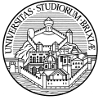
\includegraphics{Logo} 
\end{minipage}\hspace*{\fill} 

 % University/department logo - uncomment to place it

\vfill
\end{center}
\end{titlepage}

%----------------------------------------------------------------------------------------
%	ABSTRACT PAGE
%----------------------------------------------------------------------------------------

\begin{abstract}
\addchaptertocentry{\abstractname} % Add the abstract to the table of contents

%The Thesis Abstract is written here (and usually kept to just this page). The %page is kept centered vertically so can expand into the blank space above the %title too\ldots

The AEgIS Experiment at the CERN aims to verify the weak interaction principle for antimatter. This document talks about "gAnWeb", a web application designed to simplify the analysis of physical data under the AEgIS experiment. This analysis can be performed using Root Data Analysis Framework by the Linux Terminal, but a graphical interface can ensure a better user experience, eases the user training and improves the productivity. A web application is a smart way to implement the interface because allows users to avoid installations, and centralizes all the eventual modifications. This document explains the choices made during the development of this application, related to the goal of the data analysis.  

 
\end{abstract}


%----------------------------------------------------------------------------------------
%	LIST OF CONTENTS/FIGURES/TABLES PAGES
%----------------------------------------------------------------------------------------

\tableofcontents % Prints the main table of contents

%\listoffigures % Prints the list of figures

%\listoftables % Prints the list of tables


%----------------------------------------------------------------------------------------
%	THESIS CONTENT - CHAPTERS
%----------------------------------------------------------------------------------------

\mainmatter % Begin numeric (1,2,3...) page numbering

\pagestyle{thesis} % Return the page headers back to the "thesis" style

% Include the chapters of the thesis as separate files from the Chapters folder
% Uncomment the lines as you write the chapters

% Chapter 1

\chapter{Introduction} % Main chapter title

\label{Chapter1} % For referencing the chapter elsewhere, use \ref{Chapter1} 

%----------------------------------------------------------------------------------------

First of all it is important to understand at least generically what is the AEgIS experiment at the CERN and which are its goals. The acronym AEgIS stands for "Antimatter Experiment: gravity, Interferometry, Spectroscopy", this research aims to verify the weak equivalence principle for antimatter. In the first part of this chapter some particulars are explained about this experiment, in the second part is introduced gAn Web, the main topic of this document, the application that allows the physicists to do data analysis in the AEgIS experiment environment easily, through a web interface. 

\section{The AEgIS experiment}


\begin{figure}[H]
\centering

\includegraphics[scale=0.25]{aegisLogo.png} 
\caption{AEgIS's Logo}
\end{figure}

The weak equivalence principle, also known as universality of free fall, states that in the same field all bodies fall with the same acceleration, regardless of the mass and the composition. This principle has been thoroughly tested for the matter, but not for the antimatter: the most important goal of AEgIS experiment is to measure the weak equivalence principle for the antimatter; to test the universality of free fall, AEgIS will attempt to measure the gravitational interaction between matter (the Earth) and antimatter (antihydrogen). Antihydrogen is the antimatter counterpart of hydrogen, it is the simplest atom built with antimatter (see below for a description of its components). The first antihydrogen in an electromagnetic trap has been produced by the ATHENA experiment in 2012 (\url{http://www.nature.com/nature/journal/v419/n6906/full/419439a.html})
with the contribution of a group of the University of Brescia.

The AEgIS experiment is the result of a wide and international scientific collaboration, as visible in the figure 1.2.

\begin{figure}[H]
\centering 

\includegraphics[scale=0.5]{aegis_collaboration_institutes.pdf} 
\caption{Aegis Collaboration institutes}
\end{figure}


In the context of neutral antimatter, the gravitational interaction is of high interest, because it can potentially reveal new forces that violate the weak equivalence principle. Thomas Phillips, from Duke University, says: "If antimatter fell down faster, it would mean the discovery of at least one new force, probably two. If it fell up, it would mean our understanding of general relativity is incorrect". In a practical point of view AEgIS tries to measure the time of flight and the vertical displacement of antihydrogen, with a moirè deflectometer: this process is quite complex, and it is easier to explain it using the following figures (1.3, 1.4 and 1.5).

\begin{figure}[H]
\centering 
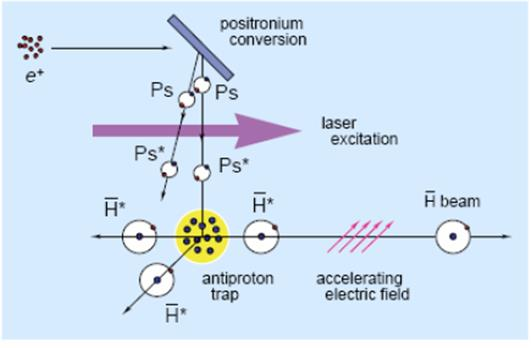
\includegraphics[scale=0.5]{AEgISScheme.png} 
\caption{AEgIS's Scheme, taken from "AEgIS experiment at CERN: measuring antihydrogen free-fall in Earth’s gravitational field to test WEP with antimatter"}
\end{figure}

In the 1.3 figure we can see the process that allows to create through a so called "charge-exchange" reaction antihydrogen. In few words, to create antihydrogen two ingredients are needed: antiprotons and positrons. The antiprotons are provided by CERN, while positrons are produced by the experiment with a radioactive source. To correctly explain this process it is better to start with some definitions:


\begin{enumerate}

% 1
\item Positron: it is the correspondent of the electron in the antimatter. It is an antielectron, that is an electron with positive electrical charge. It is indicated by "e$^{+}$".

% 2
\item Positronium: it is an unstable system consisting of an electron and a positron, bound together into an exotic atom. It is indicated with $ {Ps} $.

% 3
\item Antiproton: it is the antiparticle of the proton. Antiprotons are stable, but they are typically short-lived since any collision with a proton will cause both particles to be annihilated in a neutron and to disappear creating other particles. It is indicated with $ \overline{p} $ (pronounced pbar).

% 4
\item Antihydrogen: it is the antimatter counterpart of hydrogen. Whereas the common hydrogen atom is composed of an electron and a proton, the antihydrogen atom is made up of a positron and an antiproton. It is indicated with $ \overline{H} $ (pronounced hbar).


% 5
\item Antiproton trap: a device that uses an axial magnetic field to radially confine charged particles, in this case antiprotons.


\end{enumerate}

\begin{figure}[H]
\centering
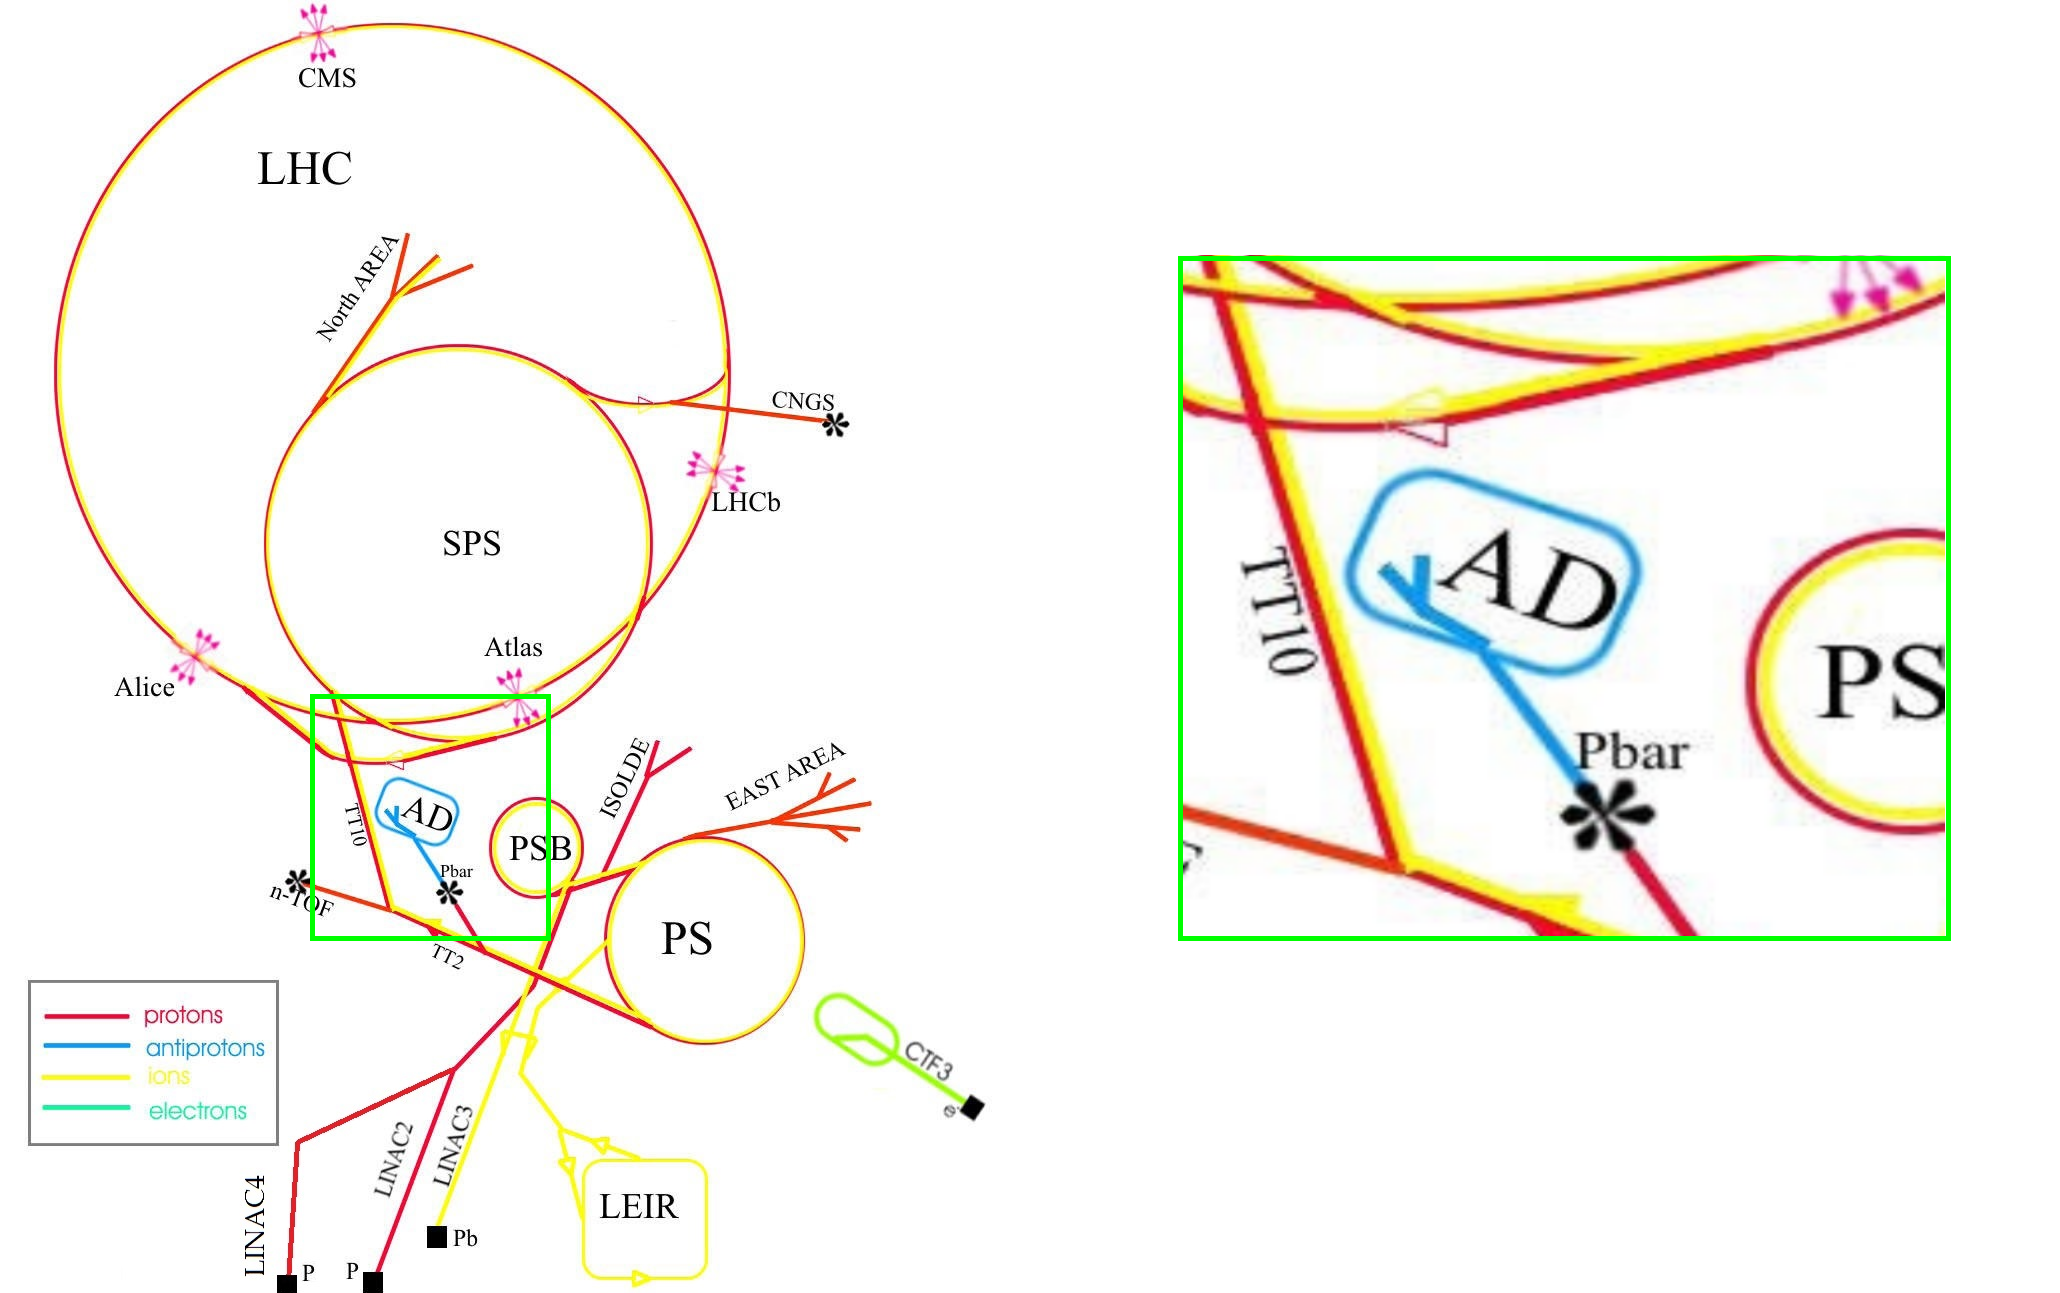
\includegraphics[scale=0.25]{CERNaccelerators.png} 
\caption{ As shown in this figure, AD in a ring in the CERN accelerator system, the AEgIS experiment is part of AD. }
\end{figure}


Antiprotons are provided by the CERN accelerator system and an electric field confines them axially. 
Protons collide with nuclei inside a metal cylinder called "target". About four proton-antiproton pairs are produced in every million collisions, and is possible to separate antiprotons using magnetic fields. The following step is to guide antiprotons toward the AD (Antiproton Decelerator, the ring shown in figure 1.4) where they are slowed down. 
The AEgIS experiment is part of AD, that is a system able to provide a stable source of antiprotons.
To execute AEgIS experiment, antiprotons must be trapped and held inside an antiproton trap, where magnetic fields force the charged antiparticles to spiral around the magnetic field lines, and electric fields confine them along the magnetic axis.

For what concerns positrons, as represented in Fig. 1.3 a beam of positrons (that comes from a $^{22}$Na radioactive source) is accelerated and driven to collide against a "positron-positronium converter" (that is a mesoporous silica film). This process creates positronium, that needs to be excited by lasers, to reach an excited state called Rydberg State. The positronium in Rydberg state is indicated by $ {Ps*} $, it has a longer life than the unexcited positronium, and can be driven to fly into an antiproton trap.


When $ {Ps*} $ is excited by lasers it can combine itself with $ \overline{p} $ to generate excited antihydrogen ($ \overline{H}* $) and electrons. The antihydrogen beam is accelerated using an electric field towards a moiré deflectometer. Then, during the travel it decays to ground state.  


\begin{figure}[H]
\centering
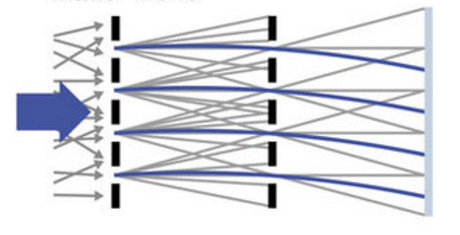
\includegraphics[scale=0.5]{MoireDeflectometer.png} 
\caption{Moiré Deflectometer's Scheme, taken from "http://www.nature.com/articles/ncomms5538" }
\end{figure}

In the Fig. 1.5 a schematic view of a moirè deflectometer is presented.
An antihydrogen beam is thrown toward two subsequent gratings that restrict the transmitted particles to well-defined trajectories. The trajectories are inflected by a force (in this case the force related to $ {m*g} $) and follow a parabolic path. At the final part of the deflectometer there is a detector that shows where the antimatter annihilates, that it is possible to compare the expected trajectories without forces with the obtained trajectories, and measure the force. The proof of principle that such system can be used with antimatter has been realized and operated with $ \overline{p} $s. It showed that a displacement of few $ \mu m $ can be detected with this technique, this result has been published in a Nature [https://www.nature.com/articles/ncomms5538]


\begin{figure}[H]
\centering
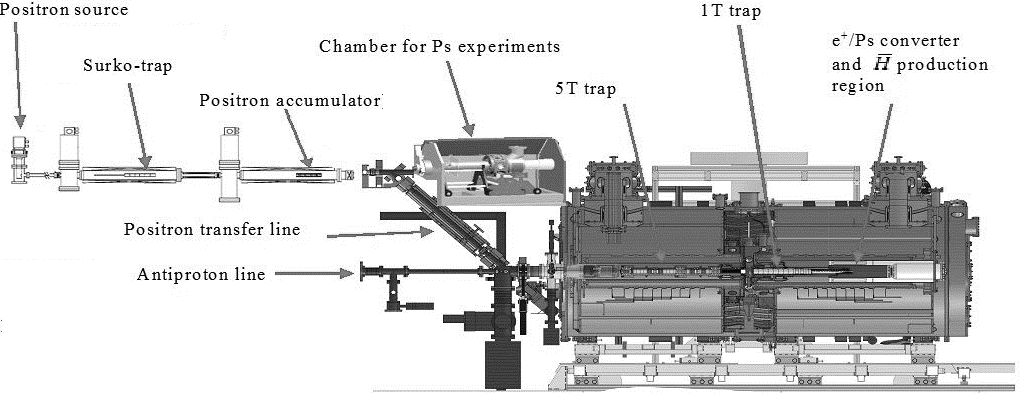
\includegraphics[scale=0.35]{SchemeMachineSetUp.png} 
\caption{AEgIS apparatus set up, taken from "AEgIS experiment at CERN: measuring antihydrogen free-fall in Earth’s gravitational field to test W.E.P. with antimatter" }
\end{figure}

% Chapter 2

\chapter{gAn, gAn Web, and their goal} % Main chapter title

\label{Chapter2} % For referencing the chapter elsewhere, use \ref{Chapter2} 

%----------------------------------------------------------------------------------------

GAn Web, is a web application, equipped with a user friendly interface, based on the most important human-machine interaction principles, designed to allow users to interact with a pre-existing data analysis application named gAn. This chapter aims to introduce information, goals, common aspects, and limits of these applications.

\section{What is data analysis?}

The main goal of gAn Web is to analyse rapidly data extracting important information, so can be useful give some preliminary information about the concept of data analysis.

According to the John Tukey's definition data analysis is: 

"Procedures for analyzing data, techniques for interpreting the results of such procedures, ways of planning the gathering of data to make its analysis easier, more precise or more accurate, and all the machinery and results of (mathematical) statistics which apply to analyzing data" 
( \url{http://projecteuclid.org/euclid.aoms/1177704711} [3]).

The basic idea is that in the modern world almost each activity can provide a big amount of data, but only a few of them are really useful to gain interesting information. The data analysis is a structured process that allows to select the most important parts of this row data and exploit them to gain information able to answer questions, test hypotheses and approve or disprove theories.
In the following figure (2.1) we can see the schema of this process. 

\begin{figure}[H]
\centering
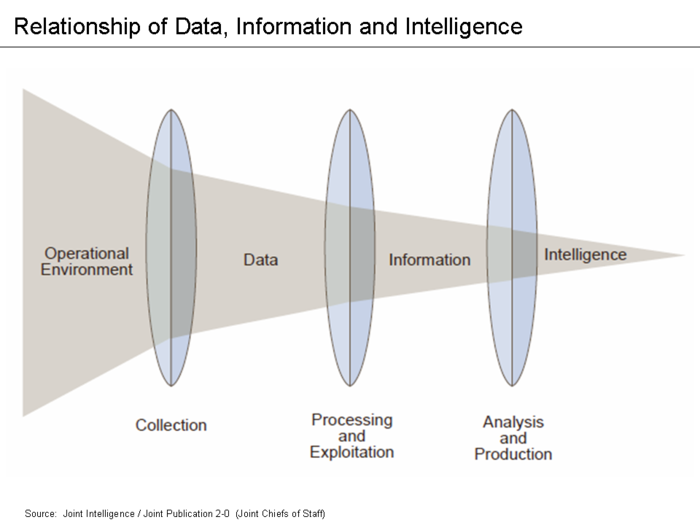
\includegraphics[scale=0.5]{DataAnalysisProcess.png} 
\caption{Here is visible a basic schema of data processes and analysis}
\end{figure}

Data analysis can be divided in some steps:

\begin{enumerate}

% 1
\item Data collection: data can be collected in a variety of ways. For example is possible to collect them using sensors in the environment, such as satellites, recording devices, physical sensors and so on. It is also possible to obtain data through interviews, downloads from online sources, or reading documentation... so the analysis is feasible with a large variety of kinds and sources of data. 

% 2
\item Data processing: raw data must be well-organized for analysis: for example, placing data into row, columns, vector, and so on (but the definition of "well-organized" in this context varies according to the kind of analysis to be performed).

% 3
\item Data cleaning: Once pre-processed and organized, the data may be incomplete, contain duplicates, or contain errors. Data cleaning is the process of correcting these errors, eliminating duplicates and handling incomplete data. Some ways to do this are record matching (comparison between the records to find if there is something suspicious), validation of data (if there is the certainty that data values has to respect some limits), overall evaluation of quality of existing data, de-duplication (process used to remove duplicates). For particular kinds of input this process is very complex (for example vocal input needs an advanced spell-checker), for others is simple (for instance online-survey interviews made using closed choices) 

% 4
\item Exploratory data analysis: in this step the data is analyzed. There are a variety of techniques referred to as "exploratory data analysis", they aim to begin understanding the real content of the data. This process may result in Descriptive statistics, such as the calculation of average or median, or in Data visualization, that allows to examine the data in graphical format, through graphics and other graphical objects.

% 5
\item Modeling and algorithms: another step is using mathematical models to find relations between different variables, such as causality or correlation. An example of this process is the regression analysis.

% 6
\item Communication: this is the final step. It is important to find a way to report the obtained information to the user in an understandable format. The communication must be adapted to the different users, in order to let the data analysis able to meet their requirements.

\end{enumerate}
According to an article written by Andrew Birmingham and Anna Russell (\url{https://which-50.com/this-is-what-big-data-}	\\ \url{really-looks-like-cern-the-universe} 	\url{-and-everything} [4]) in the particular domain of the particles physics this kind of analysis is very important: some experiments at the CERN represents about 150 million sensors delivering data 40 million times per second. There are nearly 600 million collisions per second. This is not the exactly kind of AEgIS experiment, that doesn't generate this gigantic amount of data, but, the point is that not all this information is scientifically interesting. In the huge amount of collisions discussed previously there are only around 100 collisions of interest per second.
This leads a big problem: it is difficult to find a rational way to work with flows of data having this size, and it is strongly required to take only the part of the data actually relevant for the scientific analysis, but it is also important to avoid wasting anything interesting in this dataset.

Another problem to solve to meet the user's requirements is related to the speed with which physicists develop and change focus in their experimental work: they are not interested always at the same things, and they cannot predict in advance what they will need in a remote future, because their needs are related to the process of experimentation, and can change continuously. 
Therefore a system of analysis must be very flexible and dynamic, always ready to serve to new requirements, always able to find exactly what is the "interesting" part of data.  

This kind of problems are not just CERN's problems, they are common in major research centers. Bob Jones, Project Leader at CERN, says:
"CERN is a leader but not alone in having to deal with such high data throughput. We expect to see similar scales in other sciences (such as next generation genome sequencing as well as the Square Kilometer Array which will primarily be deployed in Australia and South Africa) and various business sectors linked to the growing Internet of Things in the near future."
(quote taken from \url{http://www.cloudwatchhub.eu/what-big-data-really}	\\ \url{-looks-cern-universe-and-everything} [4])
 
Big data analysis can provide an answer to this problems: with an intelligent and parametrizable process of filtering it is possible to extract only the subset of scientifically interesting information, and delivering them to the users in an organized and structured way, by tables, statistical values, graphical images. 
In this way is possible to improve the productivity of the physicists, exempting them from unnecessary commitments and dynamically meeting their needs. 


\section{User friendly Data analysis: gAn Web}

GAn is a program that is being used to analyze data related to the AEgIS experiment at CERN, while gAn Web is the web interface to gAn, and it is the main topic of this document.

The goal of gAn Web is to allow users to perform analysis through a more friendly web interface, without install nothing on their machine. In the following image there is a schema that shows how the whole system is organized.

\begin{figure}[H]
\centering
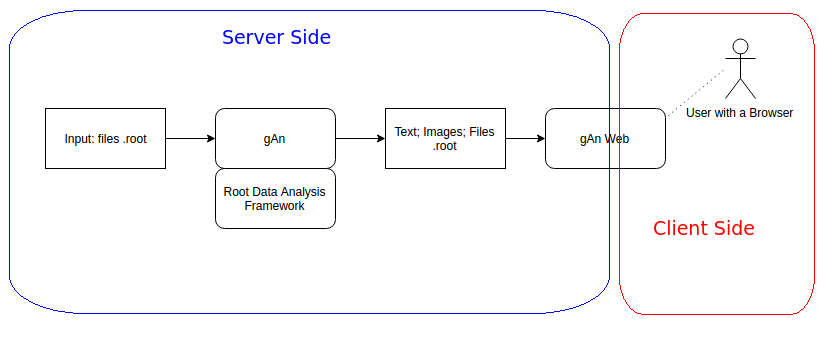
\includegraphics[scale=0.5]{GeneralGAnSchema.png} 
\caption{gAn - gAn Web simple scheme}
\end{figure}

The whole application allows to perform data collection, a process of selection and analysis of data, and data representation. In brief it means being able to extract from a big amount of raw material only the interesting information.

The raw material on which this system works is represented by a set of "Root files". 
The hardware of AEgIS experiment (mostly the detectors) generates these Root files, that are raw, binary files. 
 
The following figure (2.3) presents a schema related to the generation of these input files:

\begin{figure}[H]
\centering
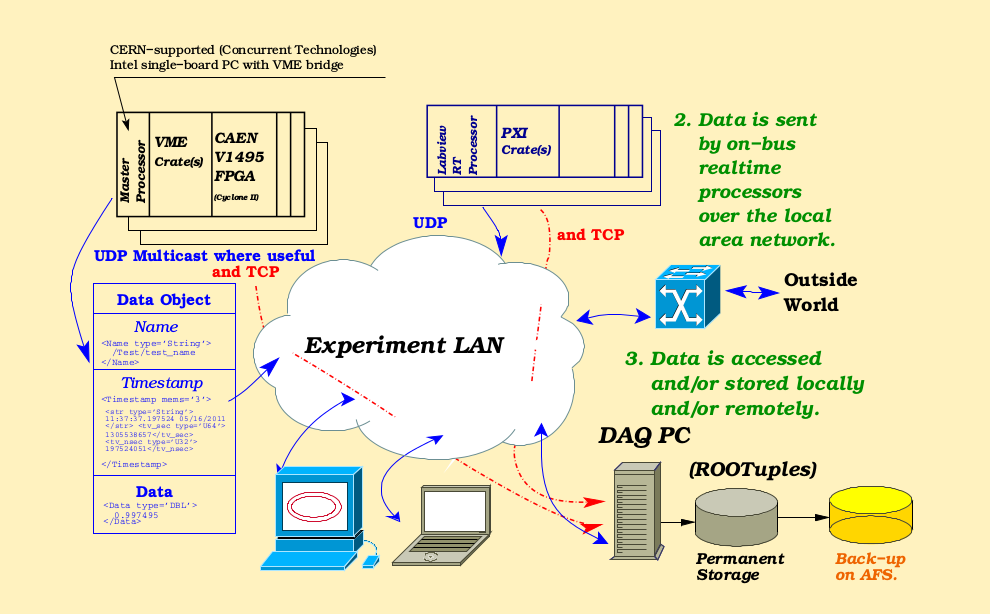
\includegraphics[scale=0.35]{DAQSchema.png} 
\caption{Root format input files generation, DAQ System}
\end{figure}

The data comes from different detectors, that communicate with different protocols, but all the communications use XML as common language. All data are sent through a LAN to a server named DAQ. Here they are stored in the root file to be ready to be analyzed.
The role of DAQ is to cover the first three steps of the data analysis process: it collects, processes and cleans data;

The Root files can be analysed using a framework named ROOT Framework, that consists in a lot of libraries specialized in high-energy physics analysis, and an interpreter able to understand a C++ script.
GAn use this framework, it can access these Root files, make an ordered and organized analysis, extract the most important information, and produce an output that consists of a text with the most important information, comments, and eventual error logs, graphic material such as images of various kind, some other Root format files, with some features used by gAn Web to make further graphical processing, related to the generation of dynamic graphics and figures. 
The goal of gAn is to reduce the big amount of raw data received in input in a little amount of scientifically interesting and easily understandable data in output, covering the forth and the fifth step of the data analysis process: exploratory analysis and modelling and algorithms.

gAn is an application developed in C++ using Object Oriented programming, making 
use of the ROOT (see Section. 2.3 for details) framework. It can be executed in a computer where ROOT 
is installed, inside the root environment with the following line command: 
\begin{verbatim}
prompt>root
root[].x rungAn.C(run_number, "analysis_file")
\end{verbatim}

where "run\_number" is a number identifying the data to be analysed (see below for a description of 
a "run") and "analysis\_file" is a string corresponding to a specific analysis on the data (each analysis
correspond to a unique analysis class, with its .C and .h files.


In order to give the correct information gAn require some inputs from the users.

The input parameters inserted by the users are:
\begin{enumerate}

% 1
\item "Run Number", that identifies in which part of the data the user is interested. 
The time in this experiment is divided in "runs" (a run lasts about some hundred seconds), so the user, by the run parameter can tell to gAn in which time slice he is interested. For example: run 55614 means that the user is interested in the information related to the 22th of November 2016, taken in the time slice between 15:45 and 15:47. 
The enumeration of the runs is incremental: so the run 55199 identifies the time slice immediately after the time slices identified by 55198. The progress of the run numbers is always going on, so new run numbers are continuously added. 
In this document every time we say "last run number" we don't mean the absolute last run numbers, but the run number that is going on right in this moment. This concept is important because usually the users use gAn Web on the last existing run number (so on the run number that is going on right at that moment) or on the immediately previous run number.  
This system used to identify time slices seems to be strange at the beginning but is a standard for all the applications in the AEgIS experiment and it allows a very efficient and precise communication. It is indeed a standard in all the experimental activities in high-energy, nuclear and particles physics. This is because inside a "run" there are data related to a specific experimental "configuration".

How can the user have more information about the runs? 
There is a RunLog (sometimes also called LogBook). The RunLog is a document organized by date on which for each run essential and specific information are reported, such as the run number, the date of acquisition, the experimental configuration, and other notes that the physicist that performed the data taking consider important to record.

% 2
\item "Type of analysis", that identifies what gAn must do with the data and what it must show as output to the user.
An analysis is basically a series of operations that treat the data to produce specific output. For example the user can look at the images regarding positrons and antiprotons and calculate the number of particles. Another example is that the user can calculate the fraction of particles that reached the end of the experiment, and so on. Each "analysis" corresponds to a specific source file that gAn loads and run accordingly.

\end{enumerate}


The output of gAn consists of a single text file with computed, (quite) organized data, and a folder of images in png format.
This structure (root files in input, data analysis using Root, images, organized and selected data in output) is very common in the CERN's experiments. 
The output of gAn is quite understandable by an experienced physicist, but it is disorganized, complex for an untrained user, and the terminal interface can be surely improved using some more user friendly technologies.

GAn Web is a web application, that aims to create a user friendly web interface, based on the most important human-machine interaction principles, between the users and gAn. 

A web interface can improve the system in two ways:

\begin{enumerate}

% 1
\item gAn is a stand-alone program based on ROOT, that can be installed on the user's machine; the user has to install the correct version of ROOT to avoid compatibility problems (ROOT is still not perfectly version independent: different versions can occasionally lead to different behaviors). Furthermore, this kind of program is continuously changing, the performed analysis is continuously improved (in the first 2 weeks from the debut of the program there were already several kinds of analysis, because often at the changing of the needs the programmers creates new analysis), so the installed version of gAn is not unchangeable, and the user must often update it. Instead, a centralized version installed on a server, with services accessible from a normal browser by the user can avoid (or at least reduce) this kind of problems and be more usable.    
 

% 2
\item a Linux terminal interface is practical for expert users, but a web based interface can be more attractive for new users, and, if well done, can be easier to use. It is important to notice that all the terminal-based applications exploit the users memory and are prone to errors.


\end{enumerate}



\section{ROOT - Physical Data Analysis }

There are some software (often free software) specialized in the analysis of data. Each of these software has strengths and weaknesses, and none of them appear to be absolutely better than the others. Following there are some examples:
 
\begin{enumerate}

% 1
\item MATLAB (matrix laboratory) is a numerical computing environment. It is a proprietary (t is not available for free, and it is quite expensive) programming language developed by MathWorks. Matlab allows matrix manipulations, plotting of functions and data, implementation of algorithms, creation of user interfaces, and embedding programs written in other languages, including C, C++, Java, Fortran and Python. 
Some detractors say that the statistical support is incomplete if compared with other solutions (also free).

% 2
\item R is a programming language and a software environment for statistical computing. It is supported by the R Foundation for Statistical Computing.The R language is widely diffused for developing statistical software and for data analysis. His popularity has increased in recent years, this is due to the fact that R is free and provides to user a good front-end interface. On the other hand some users say that the learning curve is quite hard at the beginning (in a big research center this is not a big problem..).  

% 3 
\item SciPy/NumPy/Matplotlib are libraries that work in the field of data analysis written for the general purpose language Python. It is a quite immature technology, but it is freely available and it uses a general purpose and widely diffused language like Python.

% 4
\item ROOT is an object-oriented program and library developed by CERN, released the first time in 2003 (the process of development started in 1994 and it has been continuously updated until now). It was originally designed for particle physics data analysis and contains several features specific to this field, but it is also used in other applications such as astronomy and data mining. 

\end{enumerate}

For the AEgIS experiment ROOT is the chosen software to carry out the activities of data analysis. The reason is that this software has been specifically tailored to meet the requirements of the analysis applied to particle physics.
Another advantage of ROOT is that there are a lot of libraries created during the years related to the activities of the experiments of the CERN and it is nearly impossible to rebuild them from scratch with another software.

ROOT development was started by René Brun and Fons Rademakers in 1994 (but a more extended and precise list of collaborators is accessible here \url{https://root.cern.ch/root/htmldoc/guides/users -guide/ROOTUsersGuide.html#preface} [5]). 
The ROOT's user guide start with this prefaction, that explains in detail how ROOT was born:
"In late 1994, we decided to learn and investigate Object Oriented programming and C++ to better judge the suitability of these relatively new techniques for scientific programming. We knew that there is no better way to learn a new programming environment than to use it to write a program that can solve a real problem. After a few weeks, we had our first histogramming package in C++. A few weeks later we had a rewrite of the same package using the, at that time, very new template features of C++. Again, a few weeks later we had another rewrite of the package without templates since we could only compile the version with templates on one single platform using a specific compiler. Finally, after about four months we had a histogramming package that was faster and more efficient than the well-known FORTRAN based HBOOK histogramming package. This gave us enough confidence in the new technologies to decide to continue the development. Thus was born ROOT."
(Taken from \url{https://root.cern.ch/root/htmldoc/guides/users-guide/ROOTUsersGuide.html#preface} [5])


This software is partially released under GPL (this means that everyone is allowed to use, redistribute and change the software, but any changes made must also be licensed under the GPL), and partially under LGPL (The LGPL is similar to the GPL, but is more designed for software libraries in that the developer wants to allow non-GPL applications to link to your library and utilise it).

ROOT is an object oriented framework that aims to solve problems related to high-energy physics. To better understand what is ROOT is important to start with understanding what is a framework: in IT a framework is a structure that helps the programmers providing them a set of already working utilities and services (for example, I/O, graphics, etc.) often related to the sector in which the framework aims to work (for example, the services of a web development framework are related to the layout of a web page, to the organization of DBs etc.). ROOT in particular offers services, functions, and packages related to the world of high-energy physics research, that allow to save much work.
It provides, for example the possibility to use a computer's graphics subsystem and operating system with abstraction, allowing the developer to create a graphical user interface and a GUI builder. ROOT provides also an abstract platform that allows to run C++ and command line scripts. More precisely ROOT includes (among others):

\begin{enumerate}

% 1
\item Libraries related to histogramming and graphing, that allows the developer to easily represent graphically statistical distributions. Also 3D visualization is allowed.

% 2
\item Libraries related to regression analysis.

% 3
\item Various statistics tools. 

% 4
\item Libraries related to digital image processing and manipulation.

% 5
\item Libraries aimed to allow parallel computing, (to parallelize data analysis can be really useful in order to manage the complexity of the calculations).

%6
\item The possibility of interfacing in both directions with code written in Python or Ruby.

%7 
\item The possibility of interfacing with Javascript, allowing the developer to access ROOT functionalities by a Browser.

\end{enumerate}

In the following figure (2.2) we can see the structure of the ROOT's libraries:

\begin{figure}[H]
\centering
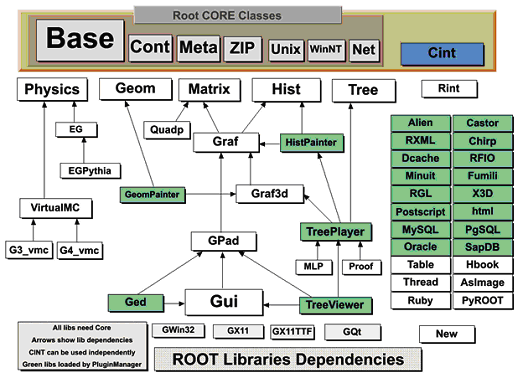
\includegraphics[scale=0.5]{RootStructure.png} 
\caption{ROOT structure}
\end{figure}


 
% Chapter 3


\chapter{User Interface } % Main chapter title

label{Chapter3} % For referencing the chapter elsewhere, use \ref{Chapter1} 

%----------------------------------------------------------------------------------------

% Define some commands to keep the formatting separated from the content 
%\newcommand{\keyword}[1]{\textbf{#2}}
%\newcommand{\tabhead}[1]{\textbf{#2}}
%\newcommand{\code}[1]{\texttt{#2}}
%\newcommand{\file}[1]{\texttt{\bfseries#2}}
%\newcommand{\option}[1]{\texttt{\itshape#2}}


\section{Human Machine Interaction principles}
todo todo

\section{Web interface vs Java Fx vs Xojo}
todo todo

\section{Used Technologies and Framworks}
todo general

\subsection{PHP}
todo particular

\subsection{Javascript}
todo particular

\subsection{Bootstrap}
todo particular

\subsection{Sass}
todo particular

% Chapter 3

\chapter{First version} % Main chapter title

\label{Chapter3} % For referencing the chapter elsewhere, use \ref{Chapter1} 


This chapter analyses which are the requirements of gAn Web at the first version and how they are implemented. This first version is very incomplete and aesthetically very raw, but very useful because it is meant to be a "test" to understand how to implement some functionalities and a base from which start to discuss with the super-users. 

\section{Functional requirements}
The definition of functional requirements aims to specifying in detail what the web application can do, and in which way an user can use it. The development of gAn Web is divided in three stages, so the requirements are peculiar and different for each stage. The first version (from now "gAn Web v1") is a very simple application: instead of access the program by a linux terminal like gAn, in gAn Web v1, the user can use the program through a graphical interface. 
The requirements of this version are the following:

\begin{enumerate}

% 1
\item The user, in the homepage, can choose the run (only one run, for the moment) in which he is interested, using an input field. This field has a validator, able to understand if the run number is inserted, if it is effectively a number, and if it is in an acceptable range. The user receives an explaining and precise error message directly on the homepage if the input field is empty or if the inserted value is not acceptable. Is it always possible validate the inserted run and ensure that the related Root file exists? No, because in some moments some sensors don't work properly and it is inevitable that some root files related to some runs are incomplete, or even in-existent. This problem will be solved in the next versions.

% 2
\item At this moment there is only a generic idea about what kind of analysis can be useful for the user, so in this version there will be only a generic analysis, able to dump in text all the possible information, and a group of example images (this is useless for the goal of the scientific research, but very useful to improve the understanding of the needed features of the web interface).
At this stage is not clear if the type of analysis will be chosen by the user of automatically selected by the program , so in gAn web v1 there are no buttons able to allow the user to select the type of analysis (this point will be reconsidered in next versions).

% 3
\item The user can start the program with a single click, by a button (usable only if the inserted number is valid).

% 4
\item When the program is executed the user can see the text output on the screen. This text is clear for a physicist (it is not clear for a person who doesn't have a specific preparation). This is an important point: there are big differences between the domain of the software engineering and the physics, so is better that this textual output is written by the hand of a physicist, to ensure to avoid misunderstanding due to different meanings assigned to symbols in different domains. Improve the legibility of the output will be a requirement for a more advanced version. 

% 5
\item When the program is executed the user can see the output images by clicking a button that link to an images-page. The images are ordered and organized by groups (the groups are related about which sensor takes the information necessary to create the image). The user can decide if he prefers to see the image in a little, medium or big format. The user can also decide if the images are distributed in the screen vertically or through a "carousel layout". The user can access the image in full-screen by clicking on it: he is redirected to a page with the image shown in full screen, and can return to the all-images page by a return button. It is absolutely important to understand exactly which information are interesting for the users, and show in the images only them and all of them, this point will be solved with a confrontation with the pilot-users. 

%6
\item The user can modify a configuration file (a .txt file on the server), by a web interface. In this file there are some values the need to be set (otherwise it uses default values), and the user can do it by radio buttons (in this way he is forced to choose valid values). This configuration file can modify the way in which gAn works and modify the resulting output (both the text and the images).   

\end{enumerate}

 
\section{Non-functional requirements}

This version (and actually also all the next versions) has some non-functional requisites:

\begin{enumerate}

\item The first is quite simple: gAn Web has to ensure that in case of crash of the program the web server mustn't crash too. The point is that on this web server (Apache server, installed on Linux) there are some other important applications, so, if gAn web crashes it is not a big problem, but the crash cannot force Apache, or worst the entire machine, to stop or restart. 
This requisite is quite easy to meet: a modern web application based on Html, Javascript, PHP and CSS is quite safe, a general crash of the server it is very unlikely to happen. If the C++ application or some Root libraries crashes (for example if the user asks for an inexistent run) the web application gracefully warn the user about the problem, but without uncontrolled behaviors.  

\item The application must work without install nothing. Also this requirement is very easy to meet: gAn Web is a web interface, it requires only a browser, nothing else.

\item The application must be compatible with any machine (except mobile phones, not requested), regardless of hardware, operating system, installed software. Also this requirement is achieved because of gAn Web only needs a browser to be used. A good observation is that the application is typically used on the computers of the AEgIS control room, that have a quite big screens, but to be sure is better to create an application able to adapt itself also to (quite) little screens.  

\item The application must be easy to be modified and extended in the future by persons who aren't necessarily software engineers. The point is that the student who wrote this program is a "momentary collaborator" in the AEgIS experiment, and all the modifications to the program must be done by other people, in most cases physicists. So the best way is to comment in detail the code and keep the code simple (this is a basic good-programming requirement).   


\end{enumerate}

\section{Scenario based functional analysis}

Following there are a list of scenarios in which a user achieves a goal by doing a list of steps. The goal of these scenarios is to show in detail how the interaction between the user and the system takes place. In this first version, the complexity of the scenarios is very low. 

\begin{enumerate}

\item The user in interested in the run 31111. In particular he is interested in the peak (the highest value) reached by a sensor named Mimito (this kind of task is very common). At this stage we still not work with kinds of analysis. The user, opened a browser in the homepage, inserts the run number and push "Send". He waits some seconds (there is a progress bar) and he arrives in a textual output page. At this point he can search in the text the information in which he is interested (it is a numerical value). Probably he is interested also in a image, to understand spatially where this peak is: he clicks on the "Show Images" button, he goes in the images pages, he selects the group "mimito", and the browser shows him a png image showing an histogram in 3 dimension: on the z-axis there is the peak, he can understand in which place (identified by x-axis and y-axis coordinates), the peak takes place, and how is shaped the resulting 3-d figure. From there he can return to the homepage and do another task.   

\item The user is no more interested in Mimito, but in another sensor: Faraday Cup. The user wants to know what are the values detected by the sensor in the same run (also this scenario is very common, often when the result of a sensor is unexpected, checking the others is interesting). This other sensor is not automatically enabled, so the user goes through the "Edit Configuration" button in a page able to modify the configuration file. Here the user can see a list of sensors, and he can use radio-buttons to modify their values from no (==disabled), to yes (==enabled). The user enables all the sensors, confirms the changes, and automatically returns in the homepage. Now he can like before insert the number, and get the outputs in textual and in images format.  



\end{enumerate}


\section{Prototyping}

This version is very simple and it contains only the basic functionalities. 
The goal of this version are: to understand if this kind of system can be useful for the users, and to experiment some technical solutions to create the features needed to achieve the goals. 

To create a prototype in this case the web programming is preferred on programs able to produce mock-ups, because the designer is quite expert in web development and can produce it quite rapidly, but he is not used to produce mock-ups with specialized software so the production of mock-ups would be slower than the complete development (actually, quite complete). 


Following are visible some part of the first prototype, with very simple features.

\begin{enumerate}
\item The homepage:

\begin{figure}[H]
\centering
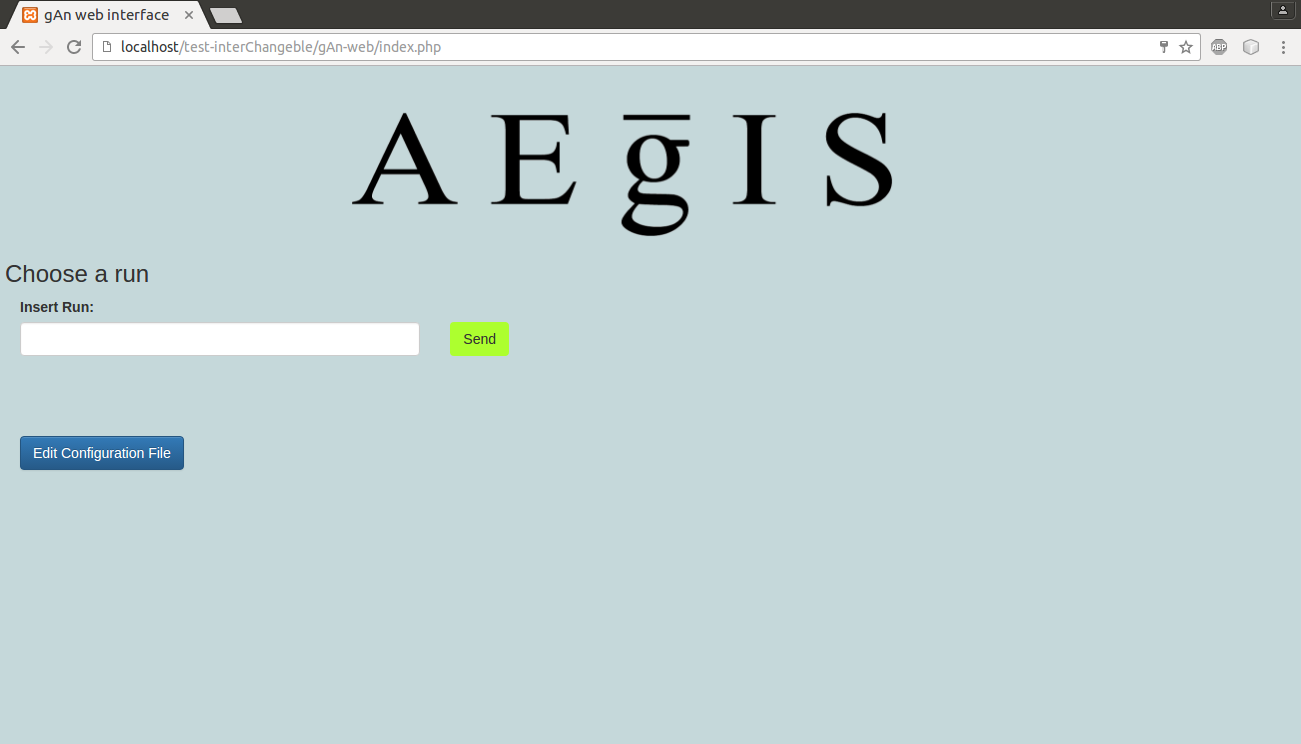
\includegraphics[scale=0.25]{HomePageOLD.png} 
\caption{First version: the first homepage of gAn Web}
\end{figure}

It is quite clear: There is the AEgIS Logo, an input field where the user can insert a run number (only one in this version) and a "Send" button to start the analysis (using gAn). A button "Edit Configuration File" allows the user to  enter in the page dedicated to the configuration of the program.

\item The text output page:

\begin{figure}[H]
\centering
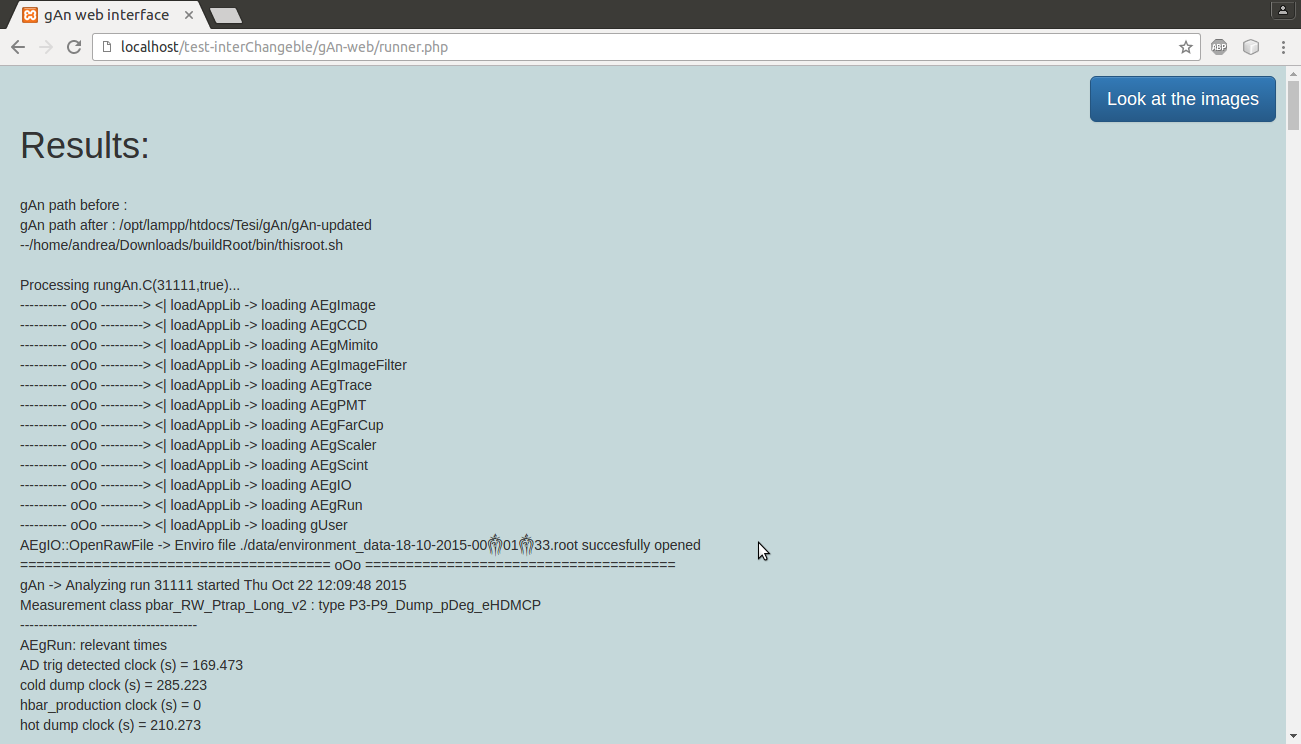
\includegraphics[scale=0.25]{TextOutputOLD.png} 
\caption{First version: the page related to the textual output of gAn Web}
\end{figure}
  
The textual result of the computation is visible: it seems to be too long and incomprehensible, but for physicists it is quite clear; to understand what is the best way to format this output a further confrontation with the users is needed. The graphics is very minimalist, there is only one button: "Look at the images", that sends the user to the page related to the images. 



\item The page related to the images:

\begin{figure}[H]
\centering
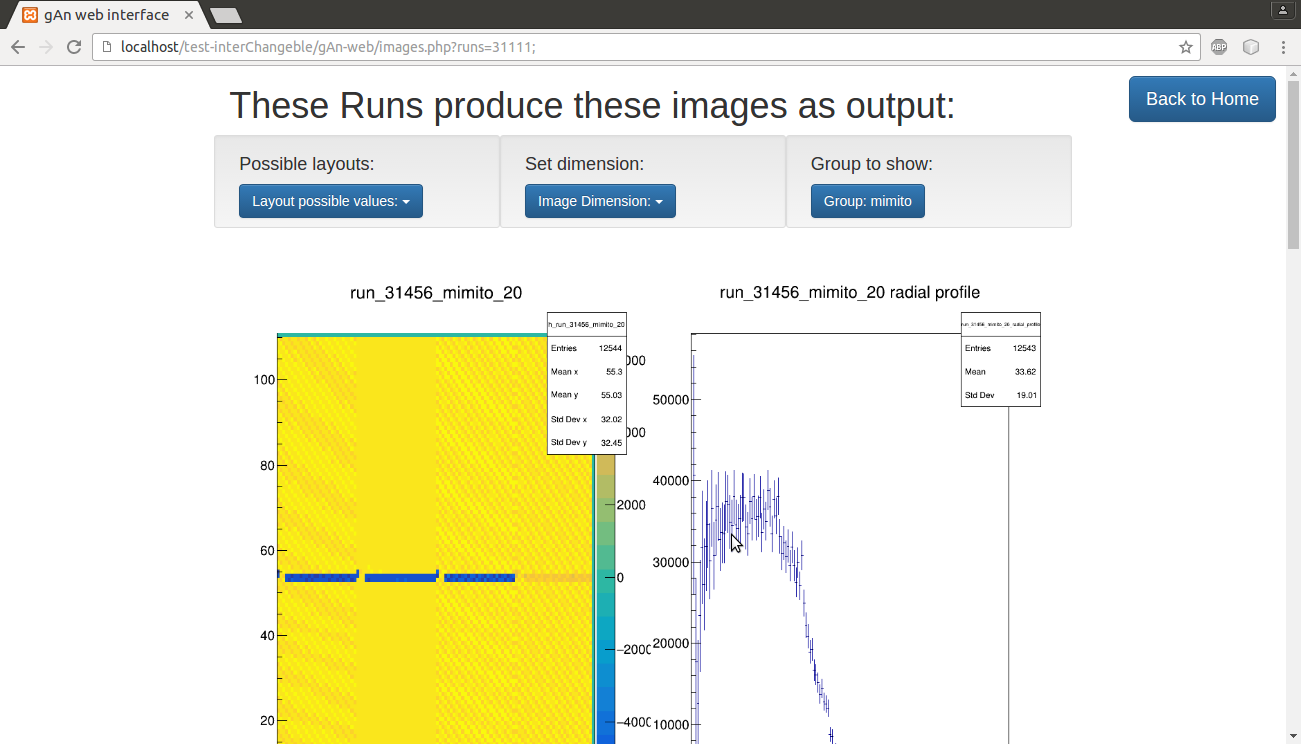
\includegraphics[scale=0.25]{AllImagesPageOLD.png}
\caption{First version: the page able to show the output images in the early prototype}
\end{figure}   

This page shows the images in a dynamic framework, that the user can edit.
The user can choose by dropdown menus the dimension, the layout ("vertical", if he prefers the images disposed vertically one above the other, "carousel" if he prefers the images organized horizontally, navigable by a "next" button and a "previous" button), the group to show (each image belongs to a group, each group usually is composed by 2-3 images). Clicking on a image the user can open it in a full page version (but it is still a static image, a png).


\item The page that aims to edit the configuration file:

\begin{figure}[H]
\centering
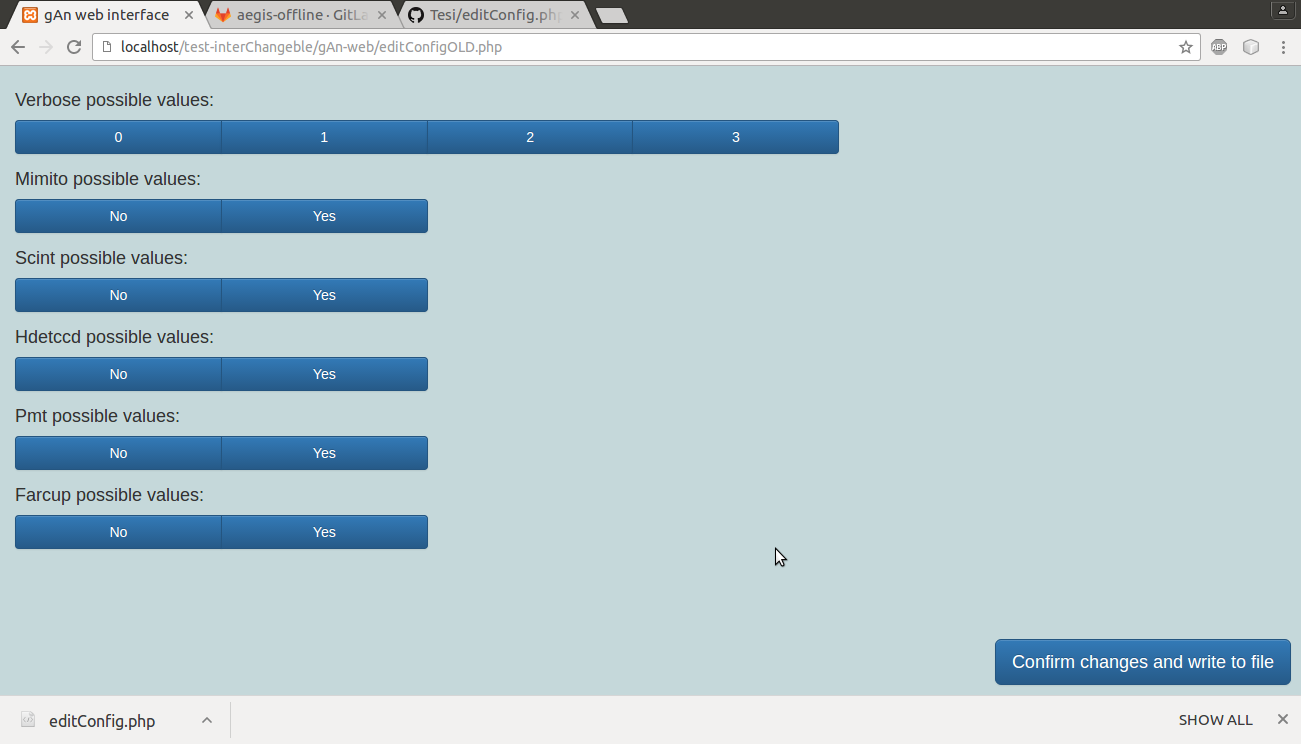
\includegraphics[scale=0.25]{EditConfigOLD.png}  
\caption{First version: the configuration page}
\end{figure}   

This page allows the user to choose by radio buttons (modified using Bootstrap graphic) the value to insert in the configuration file of gAn. Radio buttons force users to insert correct values.    

\end{enumerate}

\section{How the early version can be improved}
The early version's goal is just to be a demo. In particular, it is based on the assumption that the user knows in every moment all about gAn (how does it work,  what is the meaning of each field of the configuration file, and so on). It can be improved literally in every point, according with the principles of the Human Computer Interaction.

 
%% Chapter 5

\chapter{Intermediate version} % Main chapter title

\label{Chapter5} % For referencing the chapter elsewhere, use \ref{Chapter1} 

In this chapter the features of the intermediate version are exposed.

\section{Functional requirements}

The intermediate version (from now "gAn Web v2") is more complex than the first one. It was born from the tips and the observation of the pilot users. In this version we start to think more deeply about what functionalities are more important and how we can let them accessible by the users. The aesthetic is still not very considered at this stage (it will become important in the next stage). 
All the new required characteristics are exposed in the following:

\begin{enumerate}

% 1
\item The user can insert multiple runs: separated by a semicolon (but in case of errors the system can automatically correct them replacing symbols like "-" or "," or "." with semicolons and giving a more robust service). These runs can be inserted by an input field of by a range select button: this button opens a "modal" that allows the user to choose the first run and the last, and automatically insert the comprised runs (for example, if the user inserts 30000 and 30010 the system inserts automatically all the run numbers between 30000 and 30010). This modal has a validation system, that ensures the correctness of the inserted values. It is not perfectly clear if this solution fits the needs of the users, but the tests with the whole users group will probably solve this doubt. 

% 2
\item The user can choose which kind of analysis execute. At this point the different analysis are related to the different versions of gAn that at this stage an heterogeneous group of programmers are developing and uploading on Gitlab. It is not clear which ones of these branches will be permanent or not, so the program must be able to use all of them. The type of the analysis depends on the version of gAn downloaded and used for the execution of the program. In gAn Web v2 five complete branches exist, but in the future they may become more. They are externally very similar, the differences are the algorithms in the program, but they give a different output (different output but in the same format: text and images). 
In this version is not clear if all the different versions will be used for the final application, to clarify this point the best solution is to observe directly the user's behavior. 

% 3
\item The configuration file is not only in text format, but also can be in XML format (it depends on the selected version of gAn). The XML ensures a stronger structure, and must be transparent to the user (he doesn't see differences between the configurator that works with a txt file and the one that works with XML). At this stage both text format and XML format are acceptable, to ensure the retro-compatibility of some analysis, but it is possible that in further versions the XML-based design will become dominant. 

%4
\item The user can choose what version of Root he wants to use for the program. Theoretically different versions of Root are perfectly compatible, but in practice each version of gAn is designed to work with a particular version of Root and to avoid problems it seems to be a good idea to allow the user to choose freely among the installed versions on the server.  

%5
\item The user can save images on his hard disk: he can choose from the shown images in the images page an image to download by clicking on a specific download button near the image. Furthermore there is another button "Download All" with whom the user can simple download all the output images.

%6 
\item The user can download a reduced version of the root file with information about the images and the results: gAn produces this kind of files as "half-processed" during the computing, and it is not a problem to save this on the hard disk of the server in a specified folder. For an expert user can be scientifically interesting to have this file (this root file contains more information than the application's output, the most of this information is useless [it is an "half-processed" file] , but sometimes an expert user can find something interesting), so the user must have the opportunity to download this.     

% 7
\item The super-users prefer the dropdown menu than the radio button, so all the radio buttons in the program are replaced by dropdown menus.

% 8
\item The user has to access not only a png image, but also a root-image. This kind of image is interactive: the user can left-click and drag the mouse to select parts of the image and zoom them, and with a right click perform dynamically some kind of image processing (set colors, choose what kind of chart to show, modify the chart legend, translate in a 3D space the image etc). In this way each user can choose freely which information he wants to see in the image (try to oversee all user's needs in this part seems to be too difficult, to overcome this limit giving him the freedom of accessing the image).
All of this must be done by the user through a browser window. This requisite seems to be quite complex, but Root provides libraries (these libraries work well but they are poorly documented) to interact with Javascript.

% 9
\item In the homepage the user can see the run number of the last root file produced by the machine, and its creation date and time (so, he can understand what is the maximum of the range of the acceptable numbers). Also, the run number is an unit of measurement of the time, so through this number the user can have information about the progress of the experiment. This is an important point because actually in most cases users work with the last existing run or the one immediately before, but the way in which this application can help the user in the selection of the run needs to be deeply analyzed with a test with the users. 

% 10
\item There is a login system: the user must insert a password to use the system. The authentication is based on the comparison between the hash function of the inserted password and the hash function of the AEgIS password. If the password is correct the user receives a cookie, before each action in the site the server requests and checks this cookie to be sure about the identity of the user.  

\end{enumerate}

In the intermediate version there was another functional requirement. Ideally the user should have been able to select a gAn version also if not installed in the server machine: in this case the system should have been capable to automatically search on the AEgIS Gitlab repository the correct version (if existing), download it, unpack it in the server, and use it to execute the program. 
After some discussion this requirement has been canceled, because it was considered complex, basically useless, and potentially harmful (on the branches of the repository there are untested and incomplete versions, that can create if executed wrong outputs, so wrong scientific results). Manually installing the stable versions of gAn on the server seems to be a more smart way to work at this stage.


\subsection{Ambiguities (and related solutions)}

At least a point seems to be still ambiguous: 

The textual output of gAn needs to be formatted in some way to be more organized and clear? 
The answer is difficult: for a non-physicists this output seems to be disordered, too long, with too many groups of information, and very difficult to understand, but on this question the pilot users (that are physicists) questioned answered that the output is clear and doesn't need to be modified or improved in any way. The only requests of the users were about the font and the font-size. To check this fact the best solution probably is to observe the behavior of the users at work, and eventually ask them information about that.
Anyway, in the second version, in case of multiple run selection, there is a "navbar" that allows the user to show only a run-result per time.


\section{Scenario-based functional analysis}

In the following there is a list of scenarios able to describe samples of interaction. In this situation the interaction is more complex than before.

\begin{enumerate}

\item The user wants to analyse the runs between 30000 and 30010, plus the run 31456, to make a comparison, he is interested both in the text-output and in the images: 
the user goes to the homepage, he is redirected to the authentication page and he does the login. If the login is successful the user returns automatically in the homepage, and he can insert the runs between 30000 and 30010 manually separating them with a semicolon or better clicking the "add range of runs" button, that opens a modal, in which the user can insert the minimum and the maximum of the range, and confirm (confirmation closes the modal redirecting the user to the homepage). After the user can add manually the run 31456 separating it from the others with a semicolon. If the inserted run numbers doesn't make sense the system shows on the page an error message. If the inserted run numbers are valid, the user can click the "send" button (before the button was red and disabled, now it is green and clickable) and start gAn. A progress bar is shown, a waiting message appears, and the user waits for some seconds (at this stage of development it is very hard to predict how much time gAn requests to execute). After some seconds the user is redirected in a page that shows the textual results: on the top of the page there is a navbar that shows the computed run numbers: the user uses this navbar to choose what part of the results to show in the screen. This bar is draggable, the user can freely move it. From this page the user can, through the button "show all images", access to another page dedicated to the images. In this page he can configure through dropdown menus the dimension, the layout, the group of the images to show (each image belongs to a group, the group depends on the sensor that generates the data from that the image is generated). He can also, by clicking on a single image, access to another page, with a single image (the clicked image) that is completely accessible: the user can rotate the image, move it in a 3D space, zoom in, zoom out, select part, do some basic digital image processing and choose the kind of chart to show.   

\item The user wants to use the version 5.34 of Root (an old but stable version) to execute gAn: 
he completes the login, in the home page there is a button name "Choose Root version", clicking on this button the user is sent to a page where, he is informed about the current version of Root, and through a dropdown menu can choose among some version of Root already installed on the server (all the acceptable Root versions are installed on the server) . If the 5.34 version is one of the installed versions he can select it and confirm, the goal is achieved. If the 5.34 version is not installed, the user cannot use this version.  

\item The user wants to select the "Rug-dev" branch of gAn:
the process is very similar to the process that allows the user to choose a Root version. The user completes the login, in the home page there is a button name "Choose gAn version", clicking on this button the user is sent to a page where, he, through a dropdown menu, he can choose among some branches of gAn available on the machine. "Rug-dev" is one of these, the user can confirm and the task is completed.

\item The user wants to make the computation using only the data taken from the sensor named "Mimito":
The user, after the login, in the homepage can use the button "Edit Config" to the reach a page where, through some dropdown menus, he can change the configuration file of gAn. Each of the dropdown menus is related to a sensor (often they are 5-6, it depends on the branch), and the option of the dropdown are "yes" or "no": if "yes" is selected the sensor's data are used in the computation, if "no" they aren't. One of the dropdown menus is named "Mimito", the user select "yes" for this sensor, "no" for all the others.  

\item The user wants to download all the images related to the runs 40001 and 40002:
After the login, he can insert the runs in the homepage (it is possible both by input field and by range selector. Two ways to do the same thing: although in the next version this point will be rethought), run gAn, wait the end of the execution, click "Show all images", and from here click "download all images". All the images will be downloaded in png format.

\item The user wants to download the semi-processed root file related to the runs 31111 and 31112:
The steps are the same as the steps used to download the images, but instead of the button "Show all images", the user has to use the button "download root files".     

\end{enumerate}  


\section{Prototyping}

The intermediate version is based on the first version, but it is quite different and re-building from zero the application (re-using only some parts) is maybe the smartest solution. Some pages (and functionalities) are added, some existing pages are improved. 
Also in this case the mock-ups are interactive and really working, the developer chooses to program directly with a common web-development process HTML-javascript-PHP based, to optimize the time.

In the following all modifications are explained.

\subsection{Modified pages}
The homepage:

\begin{figure}[H]
\centering
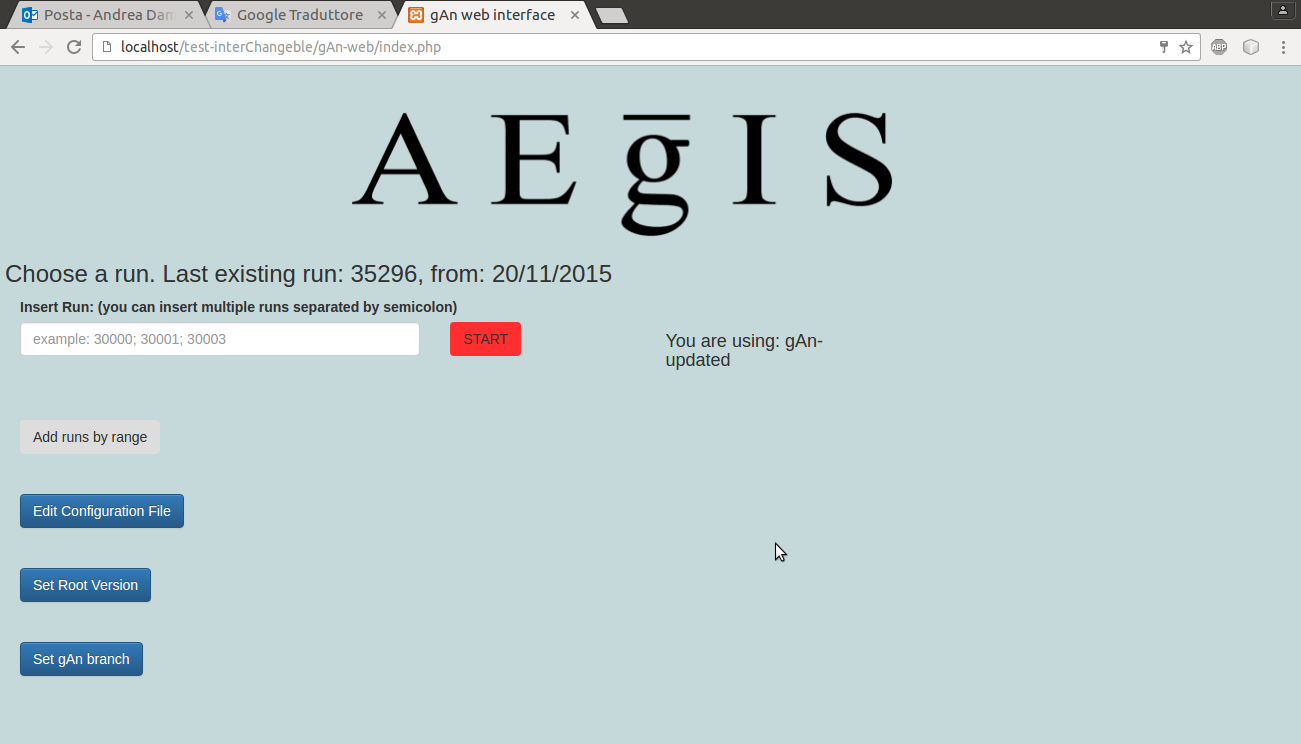
\includegraphics[scale=0.25]{HomePageEmpty.png} 
\caption{Intermediate version: the homepage of gAn Web without input}
\end{figure}


\begin{figure}[H]
\centering
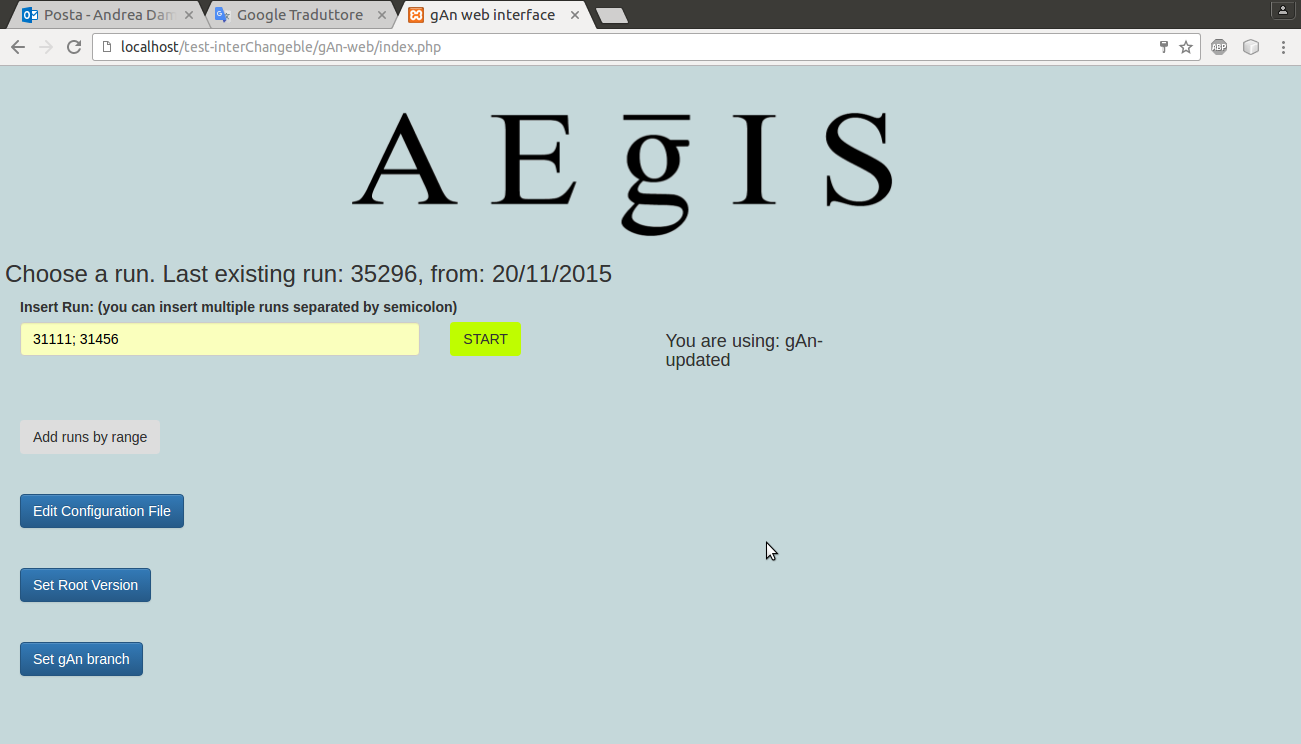
\includegraphics[scale=0.25]{HomePage.png} 
\caption{Intermediate version: the homepage of gAn Web ready to start}
\end{figure}

There are some modifications:

\begin{enumerate}

\item The user is informed about what is the last existing run: he can read "last existing run: nnnnn, from dd/mm/yy". This point is important because in most cases the user searches results regarding the lasts 2 runs.

\item The button named "send" was unclear, the word "START" is more clear, the user can immediately understand that the goal of this button is to start gAn. The button is red and disabled if there are problems (like in the following image) with the inserted runs (or if the input field is empty), green and clickable if there are no problems.	

\begin{figure}[H]
\centering
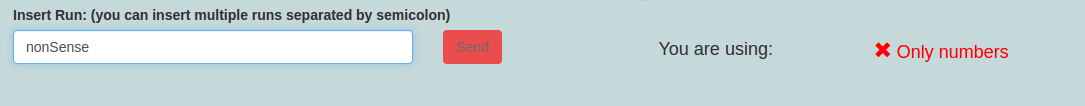
\includegraphics[scale=0.25]{ErrorInputHomepage.png}  
\caption{Intermediate version: the "Start" button is red if the values in the input field are invalid}
\end{figure}

When the user clicks start a progress bar appears. Unfortunately it is very hard to understand exactly how long the computation will last, because different runs can take different time (it depends on the amount of data that the sensors take about the run, and on the workload of the server machine, that is in common with other applications). On average has been observed that the computation takes five seconds multiplied by the number of selected runs, but there is a cache system. A wait of several seconds can be not acceptable for the user, the progress bar is imprecise but ensure to the user that the system is working correctly to ensure the correct answer. The problem is not solved: the wait time is still too long, but a solution in this case comes from the back-end, a re-factor of the code will soon make the wait time shorter. In the following image the progress bar:

\begin{figure}[H]
\centering

\includegraphics[scale=0.25]{ProgressBar.png}  
\caption{Intermediate version: the progress bar aims to make more accepttable the user's waiting}
\end{figure}



\item The input field has a place-holder, that shows to the user how to correctly insert the runs separated by semicolon (there is an automatic system that corrects the inserted values if the separator inserted by the user is not a semicolon)
 
\item It is possible to insert a group of runs selecting them by range (inserting the first and the last): the button "Add runs by range" opens a modal (shown in the image). The user can choose the minimum and the maximum value of the range, the system validates the inserted values (maximum must be more that minimum, they must be numbers etcetera).

\begin{figure}[H]
\centering
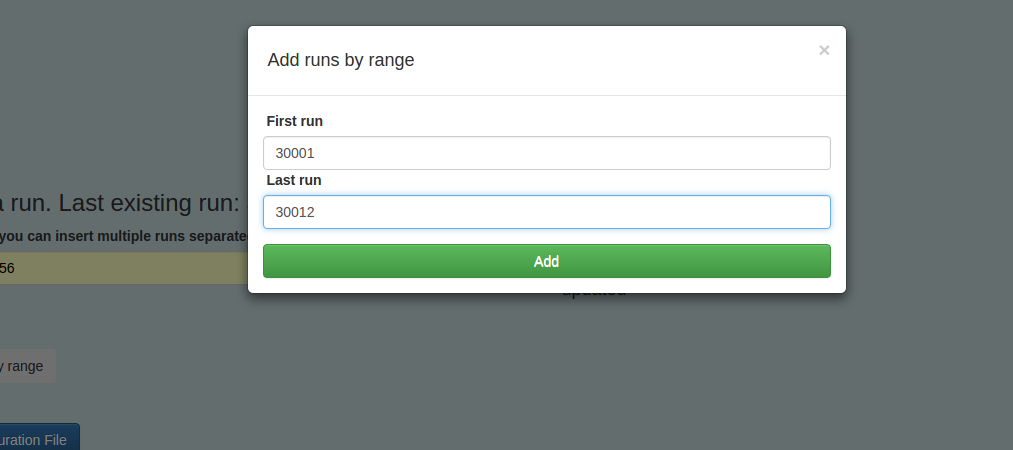
\includegraphics[scale=0.25]{RangeRunsModal.png}  
\caption{Intermediate version: the modal opened by clicking the button "Add runs by range"}
\end{figure}

\item There is a message "You are using: nameOfGAnBranch" that informs the user about which is the branch of gAn used. By default if the user doesn't change the configuration the used branch is the last used, in the last successful execution.

\item There are two new buttons: "Choose Root version", "Choose gAn version". These buttons redirect the user to pages able to modify the version of Root and gAn used in the computation.
 
\item Each button and each field have a tooltip: a text that appears when the user moves the mouse over the object. In this way an inexperienced user can easily understand what each component does.  

\end{enumerate}


The page related to the modifications of the configuration file of gAn is shown in the following:

\begin{figure}[H]
\centering
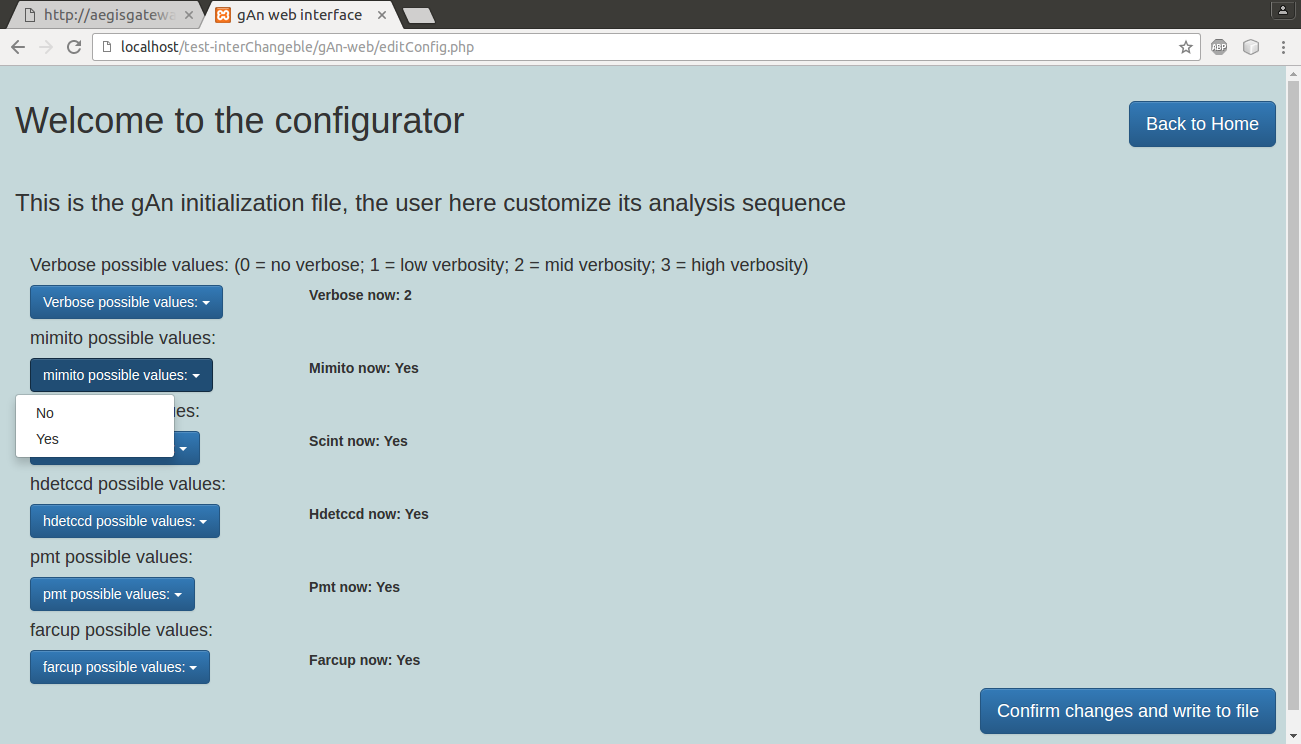
\includegraphics[scale=0.25]{EditConfig.png} 
\caption{Intermediate version: the edit-configurator page of gAn Web}
\end{figure}

This page doesn't use any more radio buttons, dropdown menus are preferred for aesthetic reasons. The user can read near the button the currently selected value for each field. 

\newpage

The page that shows the textual output of gAn is exposed in the following images, has some modifications:

\begin{figure}[H]
\centering
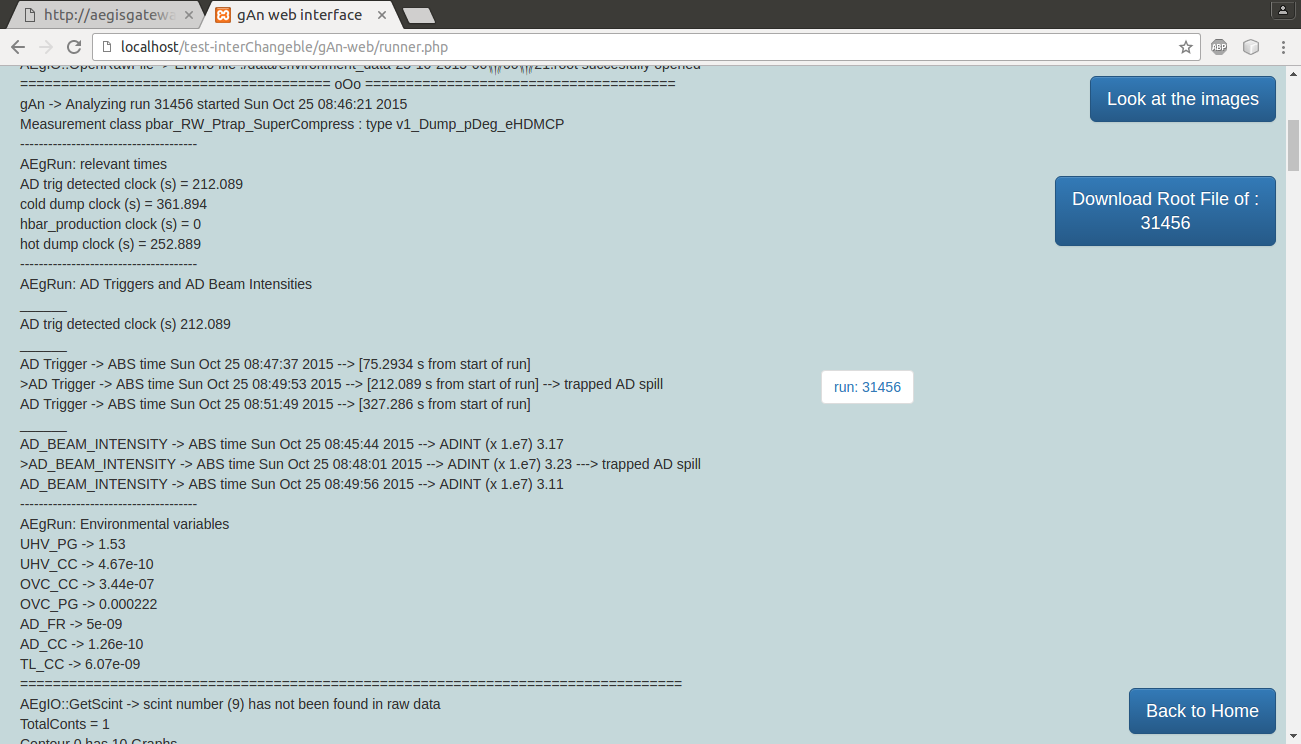
\includegraphics[scale=0.25]{TextOutputPage.png} 
\caption{Intermediate version: the page who shows the textual output of gAn}
\end{figure}


\begin{enumerate}
\item The user can choose what results he wants to show on the screen by clicking the corresponding run number from the "navbar", like in the image:

\begin{figure}[H]
\centering
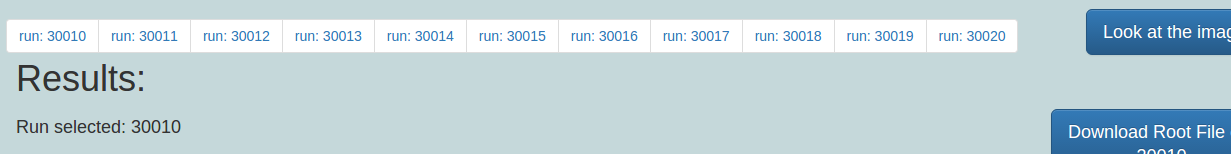
\includegraphics[scale=0.25]{WhichRunNavbar.png} 
\caption{Intermediate version: by this "navbar" the user can choose the run results to show}
\end{figure}

This navbar is in fixed position related to the screen, and can be dragged by the user to allow him to decide where put it.

\item "Download Root File of: nnnn" is a button that allows to user to download the semi-processed file .root with some output information regarding the computation.

\item "Back to Home" gives the user the opportunity to directly return to the homepage. 

\item "Back to Home" and "Look at the images" are in a fixed position on the screen: even if the user scrolls down or up the screen he is always able to see these buttons.    

\end{enumerate}
The page that shows in an organized way the images that gAn produces in output. The following image shows the new appearance of the page:



\begin{figure}[H]
\centering
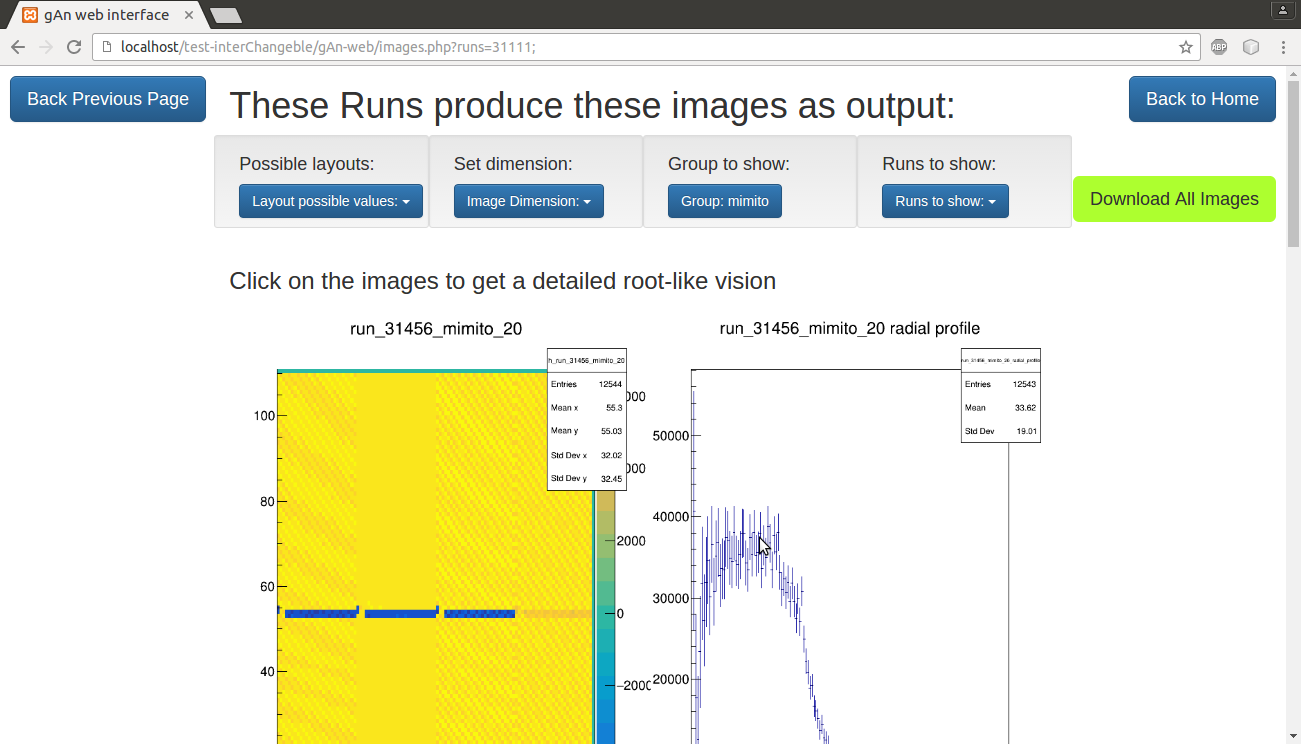
\includegraphics[scale=0.25]{AllImagesPage.png} 
\caption{Intermediate version: this page shows all the images that gAn produces in output}
\end{figure}


Modifications:
\begin{enumerate}

\item The dropdown menu "Runs to show" allows the user to select only the images produced by a single run (by default the system shows the images related to all the runs). The users widely use this option, because in this way they can compare images extrapolated in the same way but related with runs with different configurations.

\item "Download All Images" allows the user to download by a single click all the images related to the execution. The intermediate version introduces this requirement because commonly the users download the images using the right click of the mouse and the browser's button "Save Image As". In this way this process is faster and easier.

\item The buttons "Back to Previous page" and "Back to Home" are links towards the textual output page and the homepage. They are in fixed position.

\item By clicking on the image the user reaches a page that shows the image in full screen, but not in a static format: the image is dynamically accessible like shown in the following images:

\begin{figure}[H]
\centering
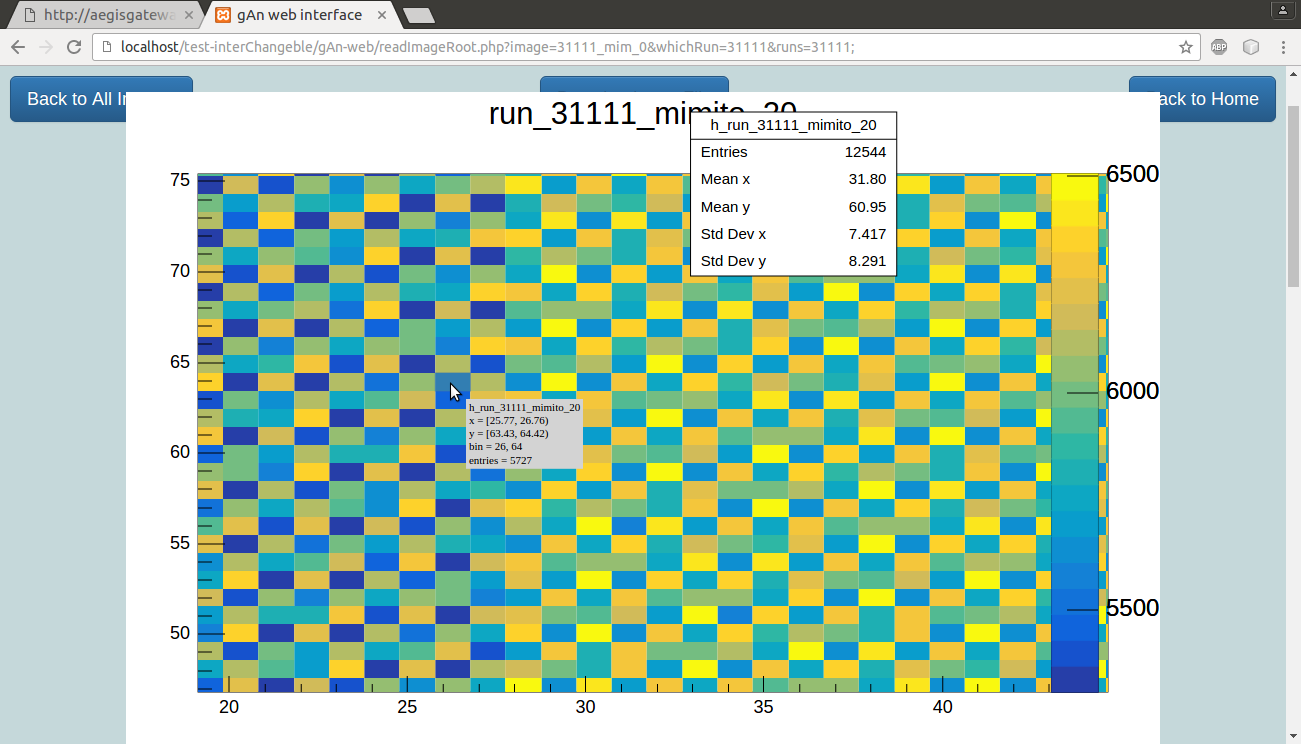
\includegraphics[scale=0.25]{RootLikeImage2.png} 
\caption{Intermediate version: moving the cursor the system shows the value of this histogram in the selected point}
\end{figure}



\begin{figure}[H]
\centering
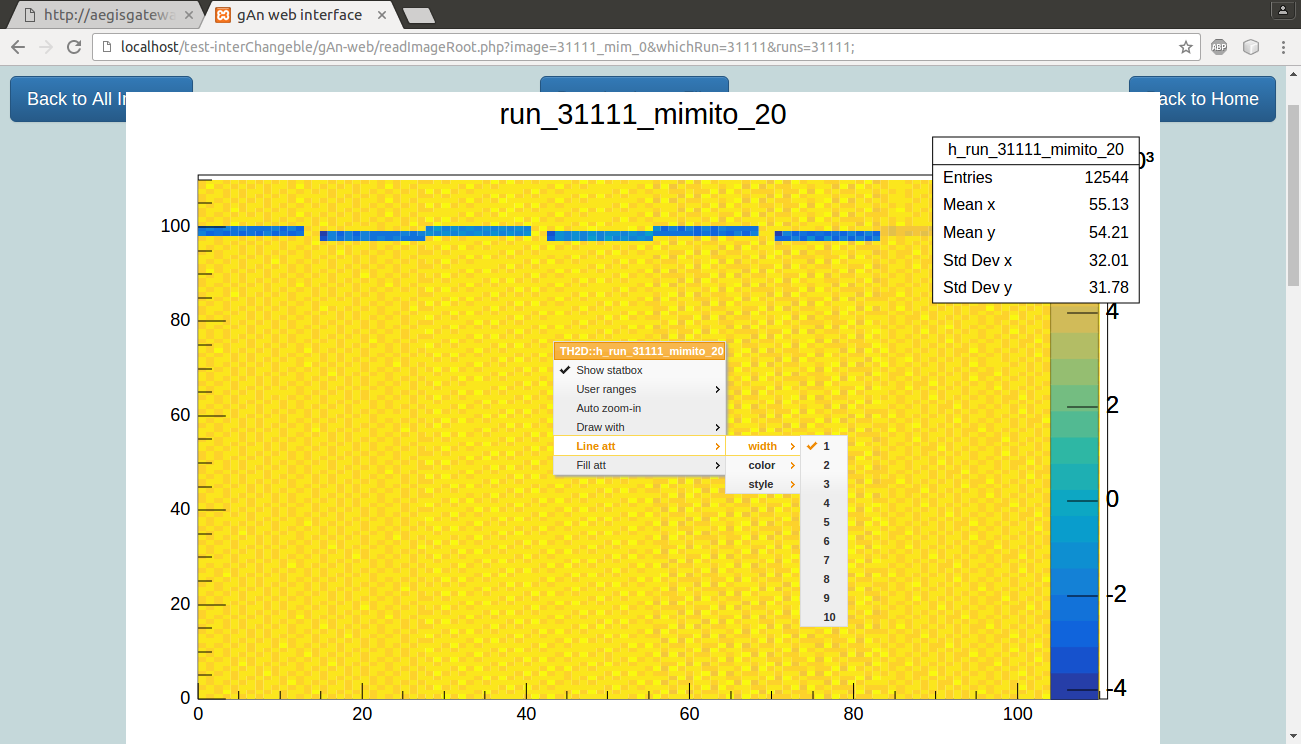
\includegraphics[scale=0.25]{RootLikeImage.png} 
\caption{Intermediate version: the user can modify numerous settings in the generated image}
\end{figure}

\begin{figure}[H]
\centering
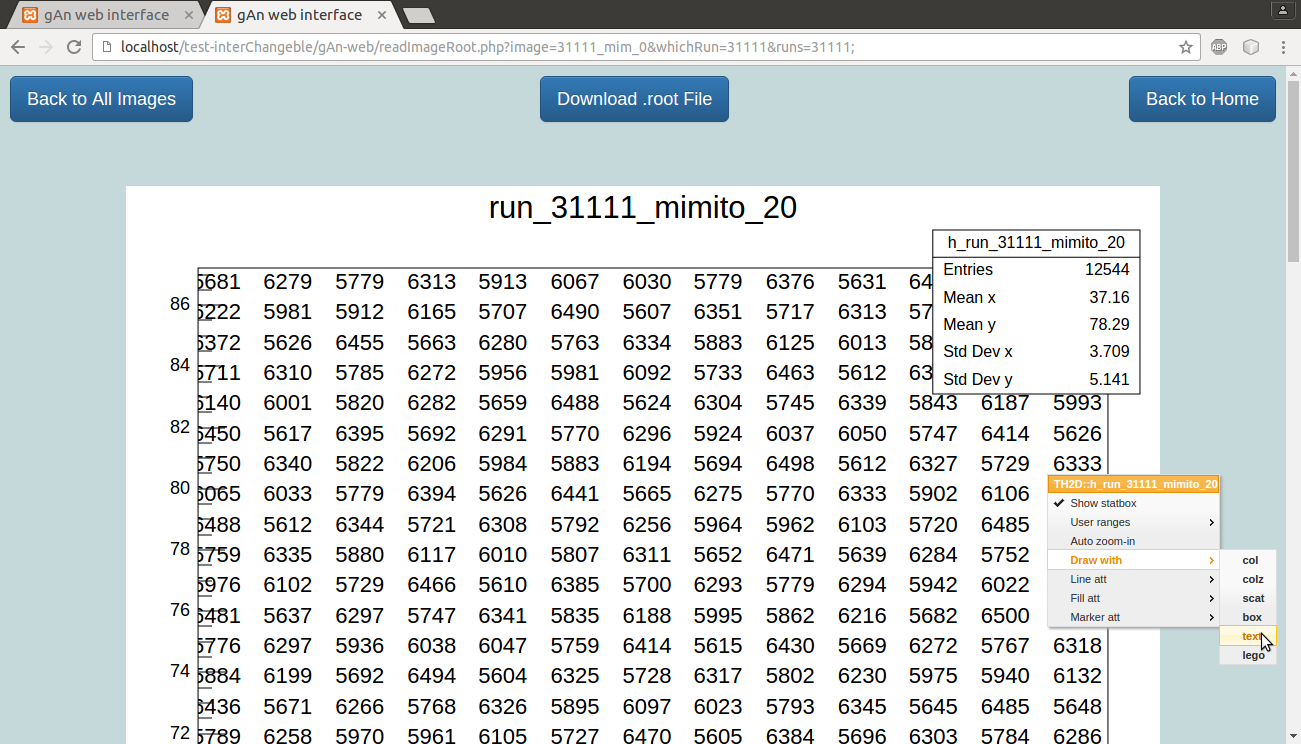
\includegraphics[scale=0.25]{RootLikeImage3.png} 
\caption{Intermediate version: the user can show the histogram not only in traditional format, but also in a numerical format where the numbers are the value of the function in their position}
\end{figure}

\begin{figure}[H]
\centering
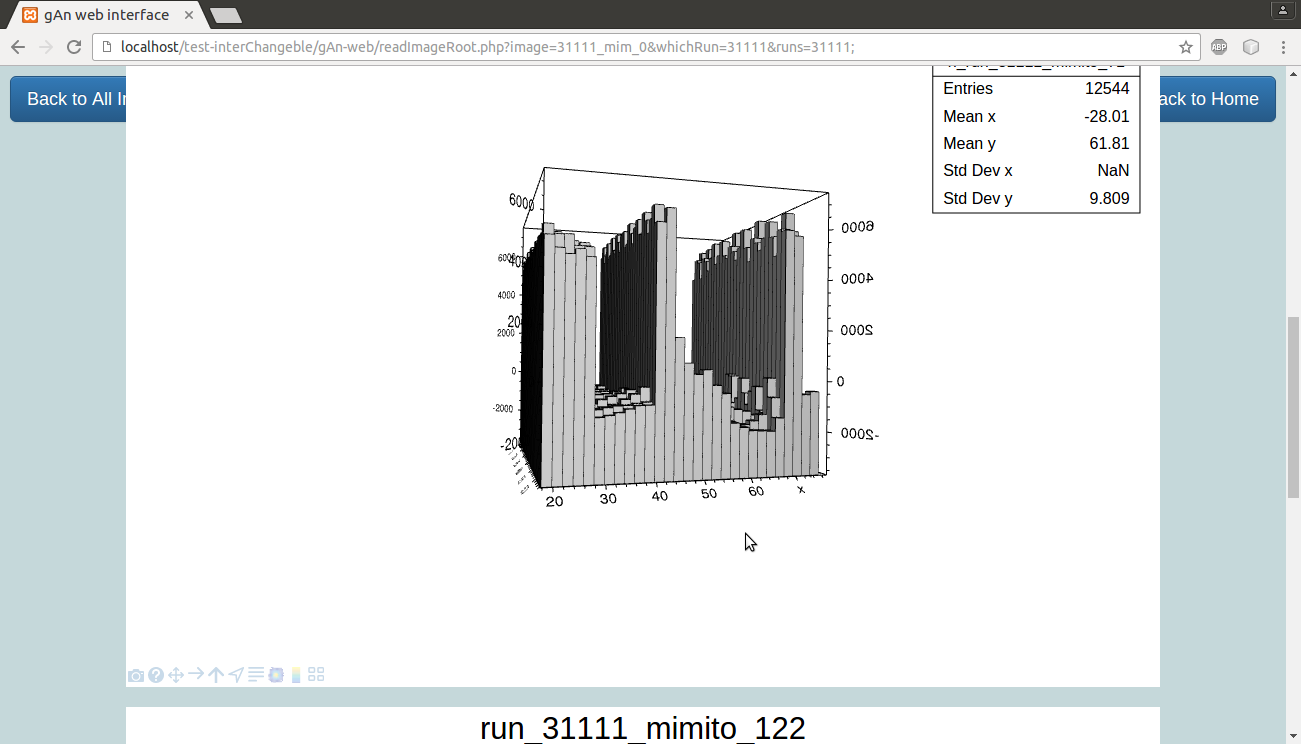
\includegraphics[scale=0.25]{RootLikeImage4.png} 
\caption{Intermediate version: another solution is to generate a 3d image in lego-style of the histogram}
\end{figure}


 
\end{enumerate}


\subsection{Added pages}

Some pages in the intermediate version are completely new, because they implement new functionalities.

The first new page that the user sees is the login page. It is very simple, it doesn't authenticate a single user, but asks only the password of the office. This basic system of authentication aims simply to ensure that only the people that works in AEgIS experiment can use this software.

Following the login page image:

\begin{figure}[H]
\centering
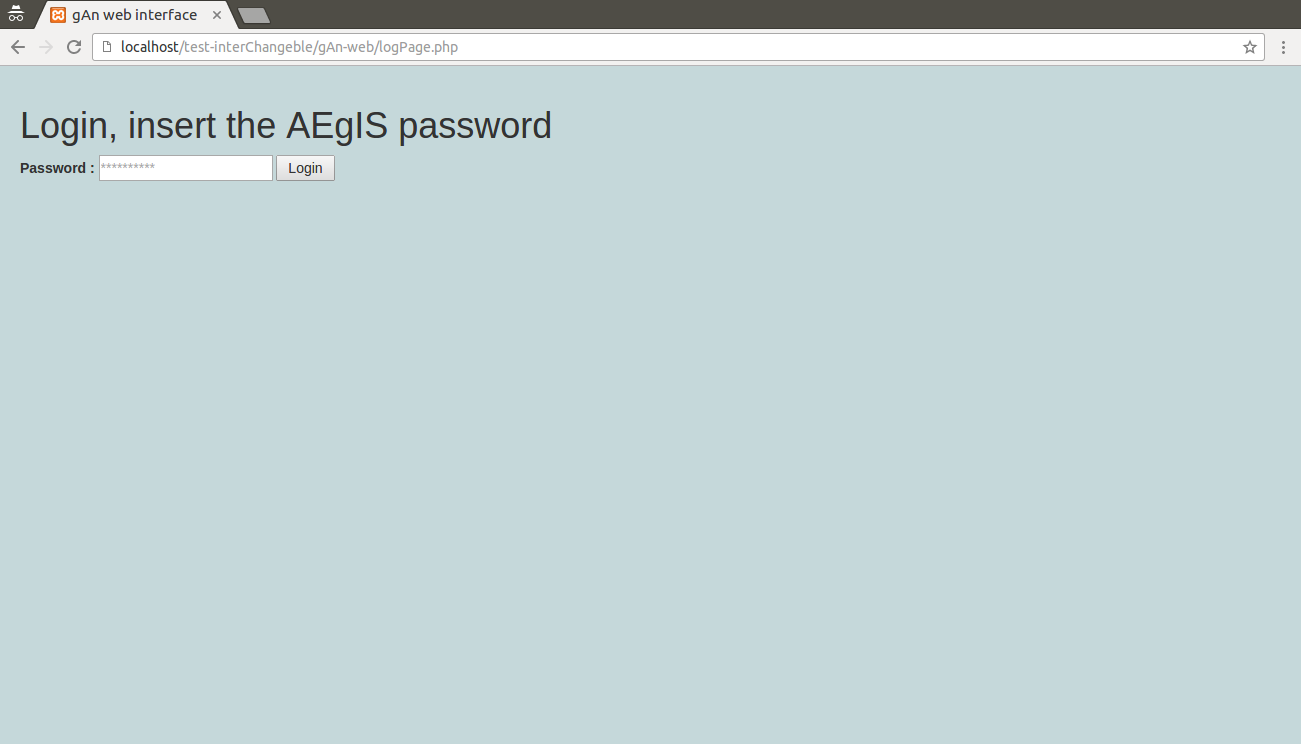
\includegraphics[scale=0.25]{Login.png} 
\caption{Intermediate version: simple login page}
\end{figure}

In this version there is also the opportunity for the user to choose which branch of gAn and which version of Root Framework to use to execute the program. The pages that the user can user are quite similar, and quite simple. The user must use dropdown menus to make these choices, and there is always a default safe choice (the system remembers the last working version of Root and the last working branch of gAn), so it is impossible make errors or inconsistent choices. 

Following there are some screen-shots of these pages

\begin{figure}[H]
\centering
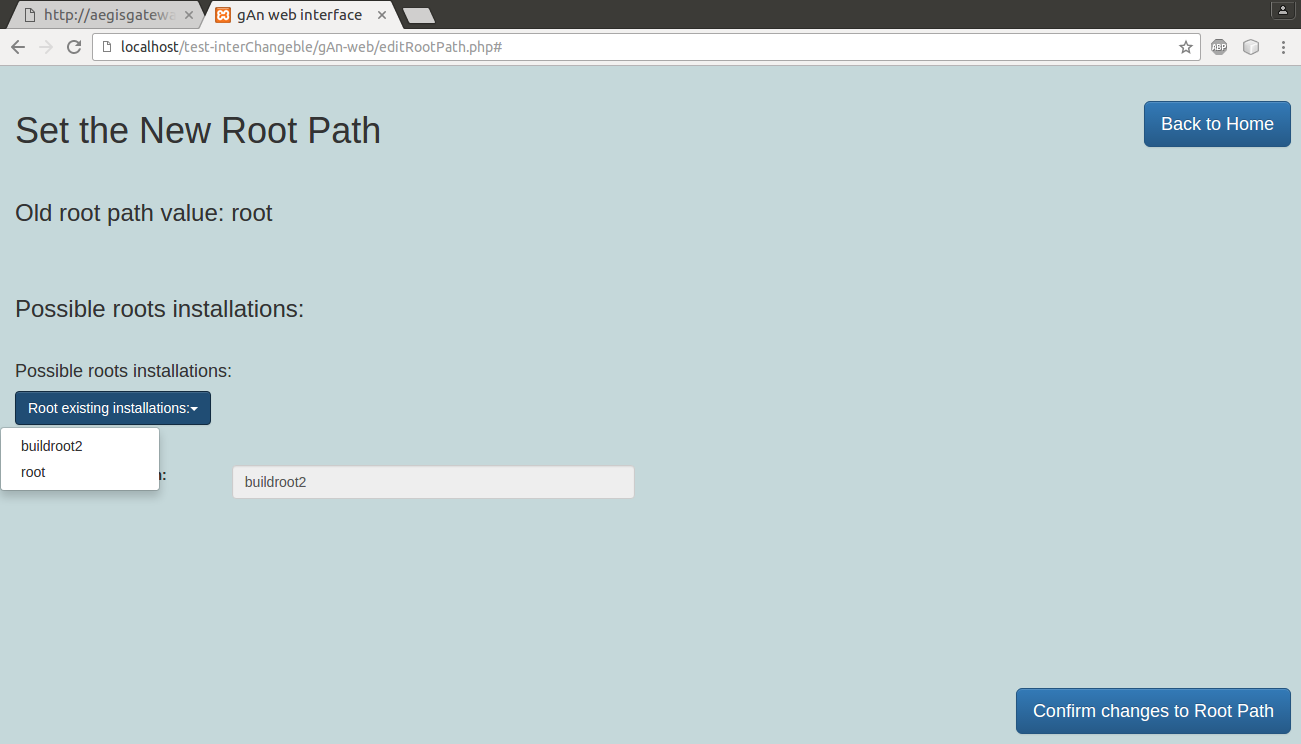
\includegraphics[scale=0.25]{RootVersionChoice.png} 
\caption{Intermediate version: page where the user can choose the Root version to use}
\end{figure}
 
 
\begin{figure}[H]
\centering
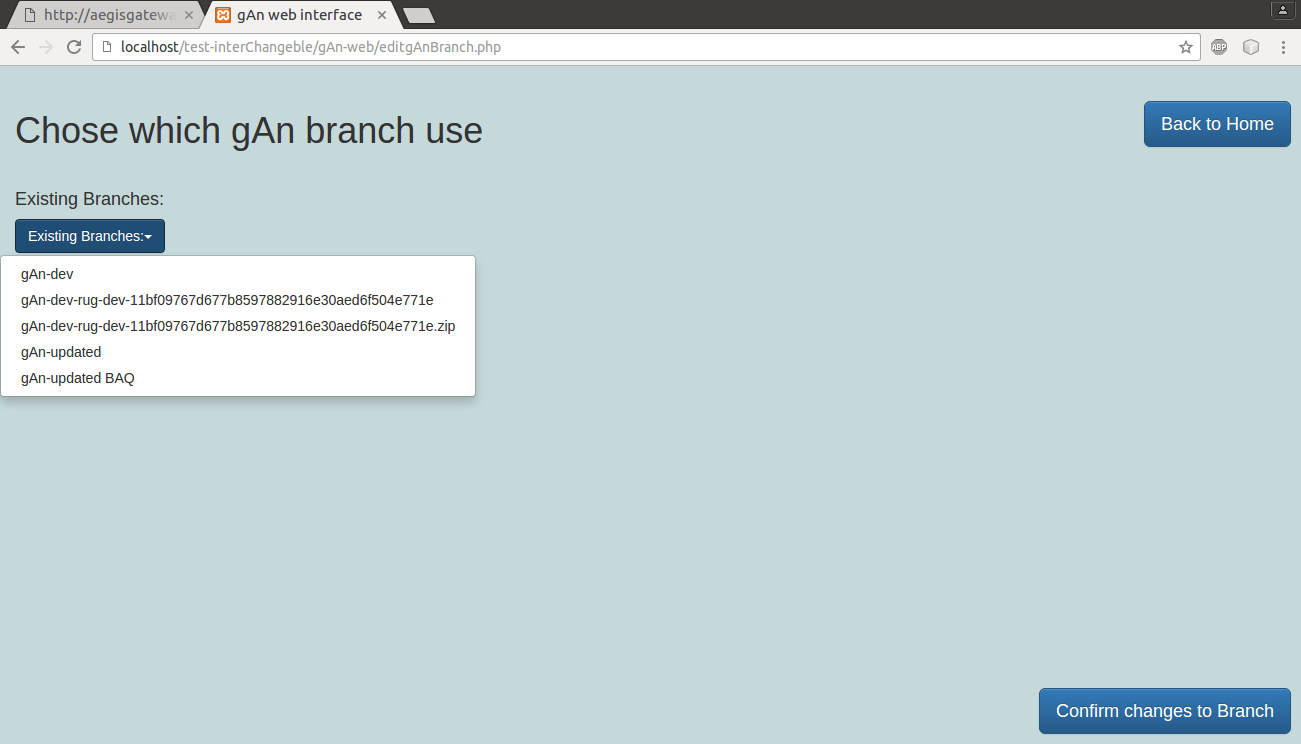
\includegraphics[scale=0.25]{ChoosegAnBranch.png} 
\caption{Intermediate version: page where the user can choose the Branch of gAn to use}
\end{figure}
 
\end{document}  
